%
% Configuratie
%

% Preambule met standaardinstellingen
\documentclass[a4paper,oneside,11pt,final]{memoir}

% Noot: zorg ervoor dat Nederlandse woord-splitsing geactiveerd is.
\usepackage[dutch,english]{babel}

% UTF8 gebruiken voor gebruik van alle symbolen
\usepackage[utf8]{inputenc}
\usepackage{eurosym}
\DeclareUnicodeCharacter{03A9}{\Omega}

% Noot: je kan het graphicxpakket een optie dvips of pdftex doorgeven
% in dat geval moet je ze ook aan iiiscriptie doorgeven, dus bijvoorbeeld
% \usepackage[dvips]{graphicx}
% \usepackage[dvips]{iiiscriptie}
\usepackage{graphicx}
\usepackage{iiiscriptie}

% Tabellen eleganter maken
\usepackage{booktabs}

% Navigeerbaarheid van hyperlinks in PDF
\usepackage{hyperref}

% Afkortingen intelligent gebruiken
\usepackage[printonlyused,withpage]{acronym}

% Math support
\usepackage{amssymb,amsmath}

% Figure wrapping (voor CC BY vermelding)
\usepackage{wrapfig}

% Listings
\usepackage{listings}
\lstset{captionpos=b, frame=tb}

% Tonen van LaTeX counters (gebruiken footnotes binnen tabel)
\usepackage{fmtcount}

% Tijdelijk uitschakelen van hyphenation
\usepackage{hyphenat}

% Extra functies
% Verkleinde margin entry
\setlength{\marginparwidth}{1.2in}
\let\oldmarginpar\marginpar
\renewcommand\marginpar[1] {\-\oldmarginpar[\raggedleft\footnotesize #1]%
{\raggedright\footnotesize #1}}

% Een TODO-entry
\newcommand{\todo}[1] {
	\addcontentsline{tdo}{todo}{\protect{#1}}
	\marginpar{#1}
}

% Hyperlink maken en URL in footnote tonen
\usepackage{hyperref}
\newcommand{\makeurl}[2]{\href{#1}{#2} \footnote{#1}}

% Compacte enumeraties
\newenvironment{enumerate_compact}{
\begin{enumerate}
  \setlength{\itemsep}{1pt}
  \setlength{\parskip}{0pt}
  \setlength{\parsep}{0pt}
}{\end{enumerate}}
\newenvironment{itemize_compact}{
\begin{itemize}
  \setlength{\itemsep}{1pt}
  \setlength{\parskip}{0pt}
  \setlength{\parsep}{0pt}
}{\end{itemize}}

% Float voor codefragmenten
\usepackage{float}
\floatstyle{ruled}
\newfloat{code}{thp}{lop}
\floatname{code}{Codefragment}


%
% Titelpagina
%

% Invullen velden
\departement{Departement Toegepaste Ingenieurswetenschappen}
\deptadres{Valentin Vaerwyckweg 1, 9000 Gent}
\studiejaar{1e Master Informatica}
\soortrapport{
Scriptie voorgedragen tot het behalen van het diploma van\\
MASTER IN DE TOEGEPASTE INGENIEURSWETENSCHAPPEN: INFORMATICA\\
}
\title{Ontwikkeling van een multimediaframework}
\bedrijfslogo{
\includegraphics[height=18mm]{logomira}}
\author{Tim BESARD}
\promotoren{
Intern:& Leen BROUNS \\
Extern:& Philippe MOLLET}


%
% Inhoud
%

\begin{document}

\frontmatter
%
% Titelpagina
%

\maketitle
\pagenumbering{roman}


%
% Abstract
%

\chapter*{Abstract}
\addcontentsline{toc}{chapter}{Abstract}
\label{chap:abstract}

%
% Voorwoord
%

\chapter*{Voorwoord}
\addcontentsline{toc}{chapter}{Voorwoord}
\label{chap:voorwoord}


%
% Inhoudstafel
%

\setlength\cftpartnumwidth{2em}

\newpage

\label{chap:inhoudstafel}
\tableofcontents

\newpage

\pagenumbering{arabic}


%
% Lijst met afbeeldingen
%

\listoffigures


%
% Lijst van afkortingen
%

\chapter*{Lijst van afkortingen}
\addcontentsline{toc}{chapter}{Lijst met afkortingen}
\label{chap:afkortingen}

\begin{acronym}[WYSIWYG]	% langste afkorting

\acro{upnp}[UPnP]{Universal Plug and Play}
\acro{mdns}[mDNS]{Multicast DNS}
\acro{dns}[DNS]{Domain Name System}
\acro{ssdp}[SSDP]{Simple Service Discovery Protocol}
\acro{dcp}[DCP]{Device Control Protocols}
\acro{ssl}[SSL]{Secure Socket Layer}
\acro{rpc}[RPC]{Remote Procedure Call}
\acro{webdav}[WebDAV]{Web-based Distributed Authoring and Versioning}
\acro{http}[HTTP]{Hypertext Transport Protocol}
\acro{rmi}[RMI]{Remote Method Invocation}
\acro{corba}[CORBA]{Common Object Request Broker Architecture}
\acro{soap}[SOAP]{Simple Object Access Protocol}
\acro{wysiwyg}[WYSIWYG]{What You See Is What You Get}
\acro{html}[HTML]{Hypertext Markup Language}
\acro{rest}[REST]{Representational State Transfer}
\acro{jvm}[JVM]{Java Virtual Machine}
\acro{svn}[SVN]{Subversion}

\end{acronym}




\mainmatter
\part{Introductie}
\label{introductie}


%
% Doelpubliek
%

\chapter{Doelpubliek}
\label{introductie:doelpubliek}

\textit{Dit hoofdstuk zal beschrijven wat er interessant is aan deze scriptie, en voor wie dat nuttig kan zijn.}


%
% Motivatie
%

\chapter{Situatie}
\label{introductie:situatie}

De volkssterrenwacht MIRA biedt zijn bezoekers een uitgebreide rondleiding over sterrenkunde en aanverwanten. Aangezien het overgrote deel van de bezoekers bestaat uit kinderen (de sterrenwacht wordt vaak in schoolverband of door families bezocht), doet men sinds jaar en dag moeite om de rondleiding zo interessant mogelijk te maken, ook wanneer er geen gids is om daarvoor te zorgen. Daartoe heeft men enkele jaren geleden een project gelanceerd, genaamd \emph{Ad-Astra}. Het doel van dit project was om multimediale kiosken te introduceren, waarbij de bezoeker via een aanraak-interface een keuze kan maken tussen verschillende multimediafragmenten. Zo staat er bijvoorbeeld bij de zaal over maanlanding een kiosk die de gebruiker toelaat om naar geluidsfragmenten van de Apollo 11 bemanning te luisteren.

Hoewel de kiosken professioneel ogen en hun werk degelijk uitvoeren, zijn er enkele problemen met het huidige systeem. De multimediafragmenten bevinden zich namelijk op een \ac{dvd} en worden verwerkt door een \acs{dvd}-speler, waarbij de gebruikersinterface bestaat uit 4 grote knoppen intern doorverbonden met de afstandsbediening.
Het grote probleem met deze opzet is de levensduur: een \acs{dvd}-speler die continu actief is, verslijt snel. Vervanging van de \acs{dvd}-speler is ook niet eenvoudig, omdat het model dat indertijd aangekocht is niet meer verkocht wordt en nieuwe modellen niet altijd compatibel zijn met de afstandsbediening in de kiosk.
Ook zijn de mogelijkheden die het systeem biedt, sterk beperkt. Alle interactiviteit moet immers geïmplementeerd worden via \acs{dvd}-menu's, wat niet veel meer toe laat dan eenvoudige selectie van het multimediafragment.

Vandaar dit project, wat de interne naam \emph{Ad-Astra III} heeft meegekregen. Voorafgegaan door Ad-Astra I (vernieuwing van de tentoonstelling) en II (vernieuwing van het telescopenpark), zal het instaan voor de vernieuwing van de museumkiosken. Het uiterlijk zal hetzelfde blijven: een kiosk zal nog steeds gestuurd worden door 4 grote knoppen, alsook zal de weergave gerealiseerd worden op een (niet aanraakgevoelig) LCD scherm, eventueel uitgebreid met een set aan luidsprekers.
Intern zal het systeem echter volledig anders werken. Een duurzame en energiezuinige chip haalt de voorstellingen op van een centrale server, waardoor het makkelijker zal zijn wijzigingen aan te brengen en die ook direct weer te geven op de kiosken. Ook zal elke kiosk continu in verbinding staan met het netwerk, wat beter beheer en weergave van dynamisch materiaal toelaat. Tenslotte zullen de voorstellingen opgebouwd zijn in een flexibel framework, wat toelaat veel rijkere inhoud weer te geven.


%
% Structuur
%

\chapter{Structuur}
\label{chat:structuur}

Deze scriptie zal beginnen met een uiteenzetting over het algemeen ontwerp in deel \ref{ontwerp}: hoe wordt het systeem gemodelleerd, voor welke technologieën is er gekozen, welke eisen worden aan de hardware gesteld, enzovoort.

Vervolgens wordt de realisatie van elk van de deelsystemen uit de doeken gedaan: de server in deel \ref{server}, de kiosk in deel \ref{kiosk}, en de ontwikkeling van de interface module in \ref{inputmodule}.

Tenslotte wordt er aandacht besteed aan de voorstellingen die het systeem zal weergeven in deel \ref{voorstellingen}. Hierbij zullen we spreken over de mogelijkheden die het systeem biedt, de code die op het prototype draait om die mogelijkheden te demonstreren, en het mechanisme dat gebruikt wordt om oudere voorstellingen zonder al te veel werk te kunnen importeren in het nieuwe systeem.

\part{Ontwerp}
\label{ontwerp}

%
% Systeemmodel
%

\chapter{Systeemmodel}
\label{ontwerp:systeemmodel}

De eerste stap van het ontwerp was de identificatie van de verschillende deelsystemen, en op welke toestellen die te vinden zijn. Hiertoe hebben we eerst gekeken naar de verschillende taken die het systeem als een geheel moet vervullen. Zo moet het systeem:
\begin{itemize}
\item Voorstellingen weergeven, en gebruikersinput verwerken;
\item Toelaten om eenvoudig voorstellingen te wijzigen, zonder veel technische bagage;
\item Voorzien in een gebruiksvriendelijke beheersinterface;
\item Dit alles voldoende robuust uitvoeren.
\end{itemize}

Hiermee konden we de verschillende deelsystemen identificeren. Zo zijn er natuurlijk de kiosken, die instaan voor de weergave van de voorstellingen, en de verwerking van gebruikersinvoer. Om het systeem flexibel te houden, zullen we de kiosken zo inrichten dat zowel de configuratie als de weer te geven voorstellingen zich niet op voorhand op de kiosk bevinden, maar van een centrale server gehaald worden. Diezelfde centrale server kan dan ook voorzien in een beheersinterface, waarbij de status van de verschillende kiosken gevisualiseerd wordt, en de administrator eventueel bepaalde acties kan ondernemen. Al deze functionaliteit zullen we bundelen binnen het specifiek hiervoor ontworpen applicatie-raamwerk, waarvoor we ook een communicatieprotocol zullen voor moeten definiëren.

\begin{figure}
	\includegraphics[width=\textwidth]{diagrammen/ontplooiingsdiagram}
	\caption{Ontplooiingsdiagram}
\end{figure}

In de volgende hoofdstukken zullen we nu elk van deze deelsystemen, en al wat daar bij hoort, tot in details uitwerken. Zo zullen we ook frequent bestaande technologieën hergebruiken, of net een gerichte keuze maken zodat hergebruik mogelijk wordt. Daarbij gaan we meestal uit van een initiële selectie aan technologieën die gebruikt kan worden om een specifiek doel te bekomen, waarna de selectie uitgedund wordt tot er slechts 1 mogelijkheid overblijft. Het valt op te merken dat we bij dergelijke selectieprocedures steeds een impliciete doch sterke voorkeur zullen stellen voor open technologieën, waarvoor er een gratis, cross-platform en open-source implementatie bestaat. Dat we kiezen voor technologieën met een kosteloze implementatie, vloeit voort uit het beperkte budget dat toegekend is door de MIRA vzw. Het cross-platform aspect is belangrijk omdat op termijn de applicatie misschien op een ander systeem zal moeten draaien, alsook het interessant zou zijn om indien het product succesvol blijkt, het open te stellen voor andere bedrijven. Het open-source kenmerk tenslotte kent zijn oorsprong weliswaar deels in idealistische gronden, maar blijkt in de praktijk ook zeer praktisch te zijn. Zo is het tijdens de realisatie van het project verschillende keren extreem nuttig gebleken om vrije toegang te hebben tot de broncode van de bibliotheek.


%
% Applicatie
%

\chapter{Applicatie}
\label{ontwerp:applicatie}

Het volgende hoofdstuk zal het ontwerp van de applicatie bespreken. Daarbij zullen we eerst de technologieën vastleggen, om vervolgens het exacte gebruik ervan te documenteren. In realiteit was dit proces echter niet zo afgelijnd: vaak leidde een bepaalde beslissing tot het terugkomen op een voorheen gemaakte keuze. In meerdere gevallen zal het dan ook voorkomen dat een specifieke eis uit het niets gegrepen lijkt, of bevooroordeeld schijnt te zijn. Toch is dit niet het geval, pas na afloop van het hoofdstuk zal het totale plaatje duidelijk worden, nadat alle beslissingen mooi in hun voegen gevallen zijn.

\section{Voorstellingen}
\label{ontwerp:applicatie:voorstellingen}

\subsection{Formaat}

Aan het formaat van de voorstellingen worden een aantal specifieke eisen gesteld:
\begin{itemize}
\item Efficiënt te distribueren over het netwerk;
\item Flexibel en toekomstgericht;
\item Terugwaarts compatibel met de huidige voorstellingen;
\item Laagdrempelig.
\end{itemize}

Zoals reeds gezegd bevinden de oude voorstellingen zich op een Dvd-schijf, in videoformaat. Het nieuwe formaat moet dus in staat zijn om video's weer te geven, eventueel na bepaalde conversies.

Na verschillende formaten vergeleken te hebben, hebben we besloten gebruik te maken van een combinatie van \ac{html} en Javascript. Die combinatie wordt vaak op het web gebruikt voor het maken van websites, en laat toe om heel dynamische voorstellingen te ontwerpen. Ook is het mogelijk om, zonder enige aanpassing aan het omliggende raamwerk, gebruik te maken van extra Javascript bibliotheken, waardoor de mogelijkheden onbegrensd zijn.

Hoewel de complexiteit enorm lijkt, zal de weergave van dergelijke voorstellingen nog relatief eenvoudig kunnen gerealiseerd worden, dit omdat \ac{html} en Javascript al jarenlang weergegeven worden binnen webbrowsers. We zullen dus de vruchten kunnen plukken van decennia aan ontwikkeling, door gebruik te maken van de \emph{rendering engines} uit verschillende browsers.

Sinds de nieuwste versie van de \ac{html} standaard, versie 5, is er ook voorzien in een \texttt{<video>} tag, die toelaat om videofragmenten weer te geven. Hierdoor voldoen we ook aan de vereiste terugwaartse compatibiliteit, al is het met enige beperkingen. Momenteel is het immers nog niet duidelijk welke videostandaard algemeen zal ondersteund worden in de \texttt{<video>} tag, meer nog, er woedt een hele strijd tussen de verschillende fabrikanten en ontwikkelaars. Afhankelijk van welke versie van welke rendering engine we gebruiken, zullen we moeten kiezen uit een andere verzameling videostandaarden.

Ook efficiënte netwerktransmissie wordt bekomen door gebruik te maken van HTML en Javascript. Alle code wordt immers opgeslagen in tekstformaat, en de videostandaarden (los van welke we uiteindelijk zullen gebruiken) zijn steeds geselecteerd wegens hun nut in context van webpagina's, waar efficiënte compressie al even belangrijk is. Wanneer men een nieuwe voorstelling ontwerpt, kan men door gebruik te maken van de vele mogelijkheden die \ac{html} versie 5 biedt, de netwerkbelasting helemaal minimaliseren. Hiertoe kunnen bijvoorbeeld binaire afbeeldingen vervangen worden door vectorafbeeldingen, en scripted animaties verkozen worden boven ordinaire videofragmenten.

Tenslotte is dit formaat voor de voorstellingen ook vrij laagdrempelig. Veel mensen hebben een basiskennis over HTML, en indien ze dit niet hebben is het eenvoudig te leren via de overvloed aan tutorials die er beschikbaar zijn. Ook is er geen nood aan een speciale \emph{toolchain}: zowel \ac{html} als Javascript bronbestanden kunnen gewijzigd worden in elke tekstverwerker, het resultaat kan eenvoudig gecontroleerd worden in een lokaal geïnstalleerde browser, en compilatie is al helemaal overbodig.
Een mogelijk probleem is de beperkte scheiding tussen design en logica: wanneer dynamiek vereist is, moet de ontwerper nogal snel enige kennis hebben van Javascript. Toch kan dit verholpen worden door gebruik te maken van \ac{wysiwyg} editors, al moet het gezegd worden dat die anno 2011 nog niet zo goed gebruik maken van alle mogelijkheden die deze nieuwe standaard biedt.

\subsection{Repository}

Zoals hierboven reeds vermeld, zullen noch de nieuwste voorstellingen noch de configuratie zich direct op de relevante kiosken bevinden, maar dynamisch van de centrale server gedownload worden. Indien voorzien wordt in een gebruiksvriendelijk systeem om de presentaties te wijzigen, maakt dit het leven van de administrator ook een pak gemakkelijker nu hij niet meer moet deployen naar elke kiosk apart.

Initieel zijn we op zoek gegaan naar een \textbf{database-systeem} om dit te implementeren. Hoewel dergelijke systemen vooral sterk zijn in het herbergen van gestructureerde data, zou het perfect mogelijk zijn om er de eerder bestandsgeoriënteerde voorstellingen in op te slaan. Efficiënte overdracht wordt echter niet voorzien, alsook zou het vrij moeilijk zijn om een gebruiksvriendelijke interface te bouwen bovenop dit systeem.

Een andere verzameling technologieën die we overwogen hebben, waren de \textbf{Enterprise Content Management} systemen. Hierbij vinden we al vaker een geïntegreerde beheersinterface, alsook komt het frequent voor dat een reeds aanwezig versiebeheer-systeem zorgt voor efficiënte dataoverdracht. Toch voldeed deze oplossing niet, daar bij dergelijke systemen de nadruk vaak nog explicieter ligt op gestructureerde data, waardoor het niet praktisch zou zijn om er onze ongestructureerde voorstellingen in op te slaan.

Daarom hebben we uiteindelijk te stap gemaakt naar gedediceerde \textbf{versiebeheer-systemen}. Hierbij is efficiënte overdracht van gegevens een basiseigenschap, alsook zorgt het bestandsgeoriënteerde aspect voor een relatief gebruiksvriendelijke interface. Zo kan een administrator heel gemakkelijk lokaal enkele wijzigingen doorvoeren aan een voorstelling, het resultaat testen in zijn browser, en indien gewenst zijn werk doorsturen naar de centrale server.

Maar er bestaan tientallen versiebeheersystemen, die we elk gepeild hebben aan ons eisenpakket:
\begin{itemize}
\item Client-server georiënteerd;
\item Efficiënte omgang met binaire bestanden.
\end{itemize}

Gezien de uiteindelijke keuze van het applicatieprotocol (zie onderdeel \ref{ontwerp:applicatie:applicatieprotocol}), komen hier nog twee eisen bij:
\begin{itemize}
\item Beveiliging via \ac{ssl};
\item Te gebruiken over \ac{http}.
\end{itemize}

Er zijn maar weinig versiebeheersystemen die aan dit eisenpakket voldoen. Meer nog, na een uitgebreide vergelijking, blijkt enkel \ac{svn} een geschikte keuze te zijn. Voor \ac{svn} bestaan er tevens Java-bindings, te vinden in de \makeurl{http://code.google.com/p/svnj/}{SVN-J} bibliotheek, waardoor de repository als 1 geheel zou kunnen geïntegreerd worden met de rest van de serverapplicatie. Jammer genoeg is de bibliotheek echter niet matuur genoeg, waardoor we zullen moeten gebruik maken van een overkoepelende webserver zoals Apache. Hierdoor wordt de binding tussen de applicatie en de repository iets minder sterk (wat bijvoorbeeld extra configuratie zal vereisen), maar het is de trade-off nodig om een realistisch systeem te bekomen.

\subsection{Repository layout}

Hoewel het nu bepaald is dat we een bestandsgeoriënteerde \ac{svn}-repository zullen gebruiken, ligt de exacte layout van de bestanden daarin nog niet vast. Aangezien zowel de voorstellingen als de kioskconfiguratie erin zal moeten opgeslagen worden, is het belangrijk om op voorhand een eenduidige structuur vast te leggen die tevens toelaat om eenvoudig wijzigingen te detecteren.

\begin{code}
\begin{verbatim}
+-repository/
  |
  +-configurations/
  | |
  | +-hires.ini
  | |
  | +-nosound.ini
  |
  +-presentations/
  | |
  | +-presentation1/
  |   |
  |   +-config.ini
  |   |
  |   +-index.html
  |
  +-kiosks/
    |
    +-kiosk1.ini
\end{verbatim}
\caption{Voorbeeld van een repository layout.}
\end{code}

Op het hoogste niveau zal de repository bestaan uit drie mappen. In de \texttt{configurations} map bevinden zich bestanden die een configuratie typeren, elk uniek geïdentificeerd door hun bestandsnaam. De configuratie bepaalt volledig hoe een kiosk zich zal gedragen. Zo wordt er voorzien in configuratiesecties voor de weergave, het geluid, het netwerk, enzovoort. Ook kan een configuratie specificeren welke voorstelling moet weergegeven worden, maar die informatie zal zich meestal bevinden in de kiosk-specifieke configuratiebstanden in de \texttt{kiosks} map. Daarin bevindt er zich een configuratiebestand per kiosk, waarin opnieuw de kiosk volledig kan geconfigureerd worden. Elk configuratiebestand (hetzij in de \texttt{kiosks} map, hetzij in de \texttt{configurations} map) kan ook specificeren welke andere configuraties tegelijk moeten ingeladen worden, waardoor gemeenschappelijke instellingen kunnen geabstraheerd worden.

De \texttt{presentations} map tenslotte bevat de effectieve voorstellingen, elk in een aparte map. In die map bevinden zich de bestanden nodig om de voorstelling weer te geven, alsook een configuratiebestand dat nu enkel specifieke eigenschappen van de presentatie configureert.

\begin{code}
\begin{verbatim}
[configuration]
description=Configuration for kiosk1.
load=nosound;hires

[presentation]
name=presentation1
\end{verbatim}
\caption{Voorbeeld van een kiosk configuratiebstand, \texttt{kiosks/kiosk1.ini}.}
\end{code}

\begin{code}
\begin{verbatim}
[configuration]
description=Configuration for kiosks without sound.

[sound]
volume=0
\end{verbatim}
\caption{Voorbeeld van een gedeeld configuratiebestand, \texttt{configurations/nosound.ini}.}
\end{code}

\begin{code}
\begin{verbatim}
description=Sample presentation 1.
landing_page=index.html
\end{verbatim}
\caption{Voorbeeld van een voorstelling configuratiebestand, \texttt{presentations/presentation1/config.ini}.}
\end{code}

\section{Applicatieprotocol}
\label{ontwerp:applicatie:applicatieprotocol}

Het applicatieprotocol zorgt voor de communicatie tussen de verschillende componenten. Omdat dit protocol instaat voor verschillende taken, zullen we dan ook gebruik maken van verschillende protocollen, elk meest geschikt voor de taak die ze moeten realiseren.

Omdat we er naar streven om geen configuratie te voorzien op de kiosken, zal een kiosk na aanmelding op 1 of andere manier moeten geconfigureerd worden. We kiezen ervoor om die configuratie uit te laten gaan van de server, die via een \textbf{remote procedure protocol} de nodige configuratiemethodes op de kiosk aanroept. Hiertoe moet bij aanmelding van een kiosk, de server een bericht krijgen, wat we kunnen realiseren met een \textbf{service discovery protocol}. Vervolgens moet de kiosk, na geconfigureerd te zijn, de data kunnen ophalen van de centrale server. De locatie van die data is doorgespeeld als onderdeel van de communicatie, en kan opgehaald worden via het \textbf{dataprotocol}.

\subsection{Beveiliging}

Ook is het vanuit bedrijfsperspectief steeds interessant om bepaalde methodes van beveiliging te overwegen. Encryptie is niet belangrijk, daar geen van de verzonden data gevoelige informatie blootgeeft. Een vorm van authenticatie is echter wel interessant, om te voorkomen dat een kwaadwillende derde de configuratie op een kiosk vervalst, of verkeerde voorstellingen publiceert. Voor het service discovery gedeelte zal blijken dat authenticatie minder belangrijk alsook moeilijk te implementeren is (het netwerk kan hoogstens vertraagd of licht verstoord worden, corruptie van gegevens is onmogelijk).

De overige twee protocollen willen we natuurlijk op een eenduidige manier van authenticatie kunnen voorzien. Hiertoe is het interessant om gebruik te maken van \ac{ssl}, een matuur en momenteel ongenaakbaar systeem van beveiliging. Bovendien kunnen we, indien beide protocollen gebruik maken van \ac{http} transport, het beveiligingsaspect louter in de overkoepelende webserver implementeren, zodat de deelprotocollen zelf geen \ac{ssl} moeten implementeren, maar toch beveiligd zijn door een robuust authenticatiemechanisme. Enkel voor clientside gebruik (wat belangrijk is voor de applicatieserver, die contact zal opnemen met een XML-RPC interface op de kiosken) is dan wetenschap van het exacte gebruik van \ac{ssl} nodig.

\subsection{Service discovery}

Service discovery is een onderdeel van de "Zeroconf" standaard, een verzameling technieken die instaat voor het initialiseren van een netwerk zonder daarbij te voorzien in expliciete configuratie. Service discovery staat daarbij in voor het ontdekken van andere toestellen, alsook eventuele services die erop aanwezig zijn. Meestal voorzien dergelijke protocollen in twee elementaire features: het \emph{publishen} van services, waarbij een toestel te kennen geeft wat zijn mogelijkheden zijn, en het \emph{browsen} van services, waarbij een toestel actief of passief op zoek gaat naar bepaalde services binnen het netwerk.

In de context van dit systeem zal een nieuwe kiosk na het opstarten zijn applicatie publiceren op het netwerk. Een eventuele server zal passief luisteren naar een dergelijke publicatie, en de informatie daarbij bekomen gebruiken om over te gaan tot configuratie van de kiosk in kwestie.

Opnieuw bestaan er verschillende technologieën die voorzien in deze elementaire functionaliteit. Opnieuw stellen we enkel bijkomende eisen om een selectie te kunnen maken:
\begin{itemize}
\item Vereist geen extra infrastructuur;
\item Cross-language implementatie;
\item Eenvoudig te gebruiken.
\end{itemize}

Een veelgebruikt protocol voor service discovery, is het \ac{ssdp}, deel van het \textbf{\ac{upnp}} systeem. Dit door Microsoft-ontwikkeld systeem, biedt een heel uitgebreid en generisch raamwerk voor service discovery, waarbij die services volledig beschreven worden door \ac{dcp}. Het geheel steunt sterk op XML en SOAP, en is strikt beheerd door het \ac{upnp} Forum. Hoewel het protocol essentieel wel voldoet aan onze eisen, is het groot en log, en biedt het veel te veel mogelijkheden die we toch niet gaan gebruiken.

Een compacter alternatief is \textbf{\ac{mdns}}, onderdeel van het door Apple ontwikkelde Zeroconf systeem. Zoals de naam doet vermoeden, is dit een multicast uitbreiding van het \ac{dns}, dat via \texttt{SRV} records toelaat om services te publiceren. Dit is een veel eleganter systeem, essentieel slechts een eenvoudige uitbreiding van een bestaande technologie, maar kent zo ook zijn tekortkomingen. Zo worden bijvoorbeeld de mogelijkheden van elke service gedetailleerd via een ongespecificeerd tekstveld. Dergelijke tekortkomingen zijn echter niet van belang in de context van dit systeem, waardoor we zullen kiezen voor dit systeem. Bovendien kent mDNS bindings voor zowel Java als Qt, de twee frameworks die we zullen gebruiken bij de effectieve realisatie van de deelsystemen (zie sectie \ref{ontwerp:applicatie:server} en \ref{ontwerp:applicatie:kiosk}).

\subsection{Remote procedure}

Van zodra de server weet heeft van een nieuwe kiosk, moet die overgaan tot de configuratie ervan. Ook moet het mogelijk zijn om acties teweeg te brengen, bijvoorbeeld ten gevolge van acties in de beheersinterface. Daarom zijn we niet op zoek gegaan naar specialistische configuratieprotocollen, maar eerder naar meer generieke \emph{remote procedure} protocollen.

Opnieuw bestaan er vele verschillende remote procedure protocollen, elk met hun specifieke eigenschappen. Grotere enterprise-projecten geven vaak de voorkeur aan technologieën zoals \textbf{\ac{soap}} of \textbf{\ac{corba}}, enorme systemen die zeer uitgebreide mogelijkheden kennen. We zullen dergelijke technologieën echter om dezelfde reden vermijden als waarom we \ac{mdns} boven \ac{upnp} verkozen hebben: in de context van dit project is een compacter en eleganter protocol veel beter te controleren en dus interessanter dan een complex te configureren alleskunner waarvan de helft van de mogelijkheden toch onbenut blijven.

In de categorie van compactere RPC-protocollen vinden we zo bijvoorbeeld \textbf{\ac{rest}}. Hoewel dit lichtgewicht, \ac{http}-gebaseerd, en ook vaak gebruikt protocol op het eerste zicht aan onze eisen voldoet, kent het zijn mindere kanten. Zo kent het geen eenduidige manier om fouten terug te geven, alsook is het formaat waarin data verstuurd wordt niet gestandaardiseerd. Omdat het manueel voorzien van deze mogelijkheden nog vrij veel werk zou innemen, besteden we verder geen aandacht aan dit protocol.

De meest courante ontwikkelframeworks zoals .NET en Java kennen meestal ook hun eigen \ac{rpc}-protocol, zoals \textbf{.NET Remoting} en \textbf{\ac{rmi}}. Hoewel deze protocollen meestal vrij matuur en veelzijdig zijn, zijn ze vaak niet cross-platform en zeker niet cross-language, waardoor ze tevens afvallen.

Ook hebben we meer moderne \ac{rpc}-frameworks overwogen zoals \textbf{Apache Etch}, of \textbf{Apache Thrift}. Deze vrij nieuwe en tevens veelbelovende systemen bleken echter enkele kritieke eisen mis te lopen. Zo kent Apache Etch slechts een beperkte verzameling language bindings, en kent geen van beide een authenticatiemechanisme. Omdat beide verlopen over een eigen protocol, vallen ze ook niet te overkoepelen onder een SSL webserver.

Daarom hebben we uiteindelijk gekozen voor \textbf{XML-RPC}, een zeer simplistisch \ac{rpc}-protocol dat XML-geformatteerde berichten verstuurd over \ac{http} transport. Hierdoor wordt het mogelijk om op een transparante manier een vorm van authenticatiecontrole toe te voegen. Toch kent XML-RPC ook zijn fundamentele problemen, zoals het inefficiënte berichtformaat. Omdat we berusten op een apart dataprotocol, is dit echter geen groot probleem. Ook is de specificatie, zacht uitgedrukt, vrij beperkt. Dit kan echter een voordeel zijn: de ermee geïmplementeerde interface wordt er compact mee gehouden, en valt eenvoudig te gebruiken vanuit verschillende talen. Dit wordt ook vereenvoudigd door de uitgebreide waaier aan implementaties, die er voor quasi elke taal is.

\subsection{Data uitwisseling}

In eerste instantie was het niet de bedoeling gebruik te maken van een derde deelprotocol, maar om de data te versturen over het \ac{rpc} protocol. Na enig onderzoek bleek echter dat zowel het gebruik van een geïntegreerd datasysteem (zie \ref{ontwerp:applicatie:voorstellingen}), als het integreren van een versiebeheersysteem, niet zou lukken.

Nu voorzien we echter in een apart versiebeheersysteem (\ac{svn}), dat vaak gebruikt wordt in aaneenschakeling met een webserver. Hierbij wordt het de communicatie bekomen over het \ac{webdav} protocol, dat tevens over \ac{http} getransporteerd wordt. Dit laat ons opnieuw toe op eenvoudige wijze authenticatie toe te voegen, alsook ontlast het ons \ac{rpc} protocol van de effectieve dataoverdracht.

\section{Redundantie en robuustheid}
\label{sec:redundantie}

Een belangrijk aspect van het systeem is dat het robuust is, en dus voorziet in een bepaalde vorm van redundantie. Zoals het hardwareontwerp zal verduidelijken (zie hoofdstuk \ref{ontwerp:hardware}), voorzien we reeds in hardwarematige redundantie onder de vorm van een RAID opstelling. Toch verhelpt dit het fundamentele probleem niet: de centrale server is een \emph{single point of failure}.

Een eerste idee om dit te verhelpen was het voorzien van een \textbf{backup server}, die de centrale server continu zou monitoren. In geval van diens falen, zou de failover functionaliteit geactiveerd worden, waarbij de taken van de centrale server integraal overgenomen zouden worden. Gezien het configuratieloze aspect van de opstelling, en het feit dat elk initiatief steeds van de servers uit komt, zou dit totaal geen actie vereisen. Om ervoor te zorgen dat de backup server steeds over de meest recente informatie beschikt, activeert die tevens een (passieve) \ac{mdns} module, alsook registreert die zich bij de primaire server zodat updates aan de presentatie-repository steeds op beide servers aanwezig zijn.
Hoewel deze configuratie zeer elegant lijkt (zeker indien de replicatie alsook promotie/degradatie van de server volledig autonoom verloopt), is ze niet realistisch op budgettair vlak. Het is niet alleen kostelijk om een tweede voldoende krachtige server samen te stellen, maar de aanwezigheid ervan betekent een extra continue energieconsumptie.

Daarom hebben we gekozen voor een tweede piste, namelijk het gebruik van een \textbf{backup-cache in de kiosken}. Aangezien embedded hardware vaak komt met een optie voor een kaartslot, is het voordeliger om voor elke kiosk een dergelijke geheugenkaart aan te kopen, en de applicatie te voorzien van de functionaliteit om bij het opvragen van de configuratie en voorstellingen die lokaal op te slaan. Wanneer vervolgens de centrale server onbereikbaar blijkt te zijn, kan steeds gebruik gemaakt worden van deze lokale cache om toch volwaardig te kunnen blijven functioneren.

\section{Server}
\label{ontwerp:applicatie:server}

Zoals reeds vermeld, is de centrale server van essentieel belang in het systeem. Zo verzorgt de server:
\begin{itemize}
\item Configuratie van de kiosken;
\item Opslag en distributie van de voorstellingen.
\end{itemize}

Naast deze elementaire taken, vereenvoudigd de server tevens de werklast van een administrator. We zullen immers voorzien in een beheersinterface die niet alleen een overzicht van het systeem biedt, maar ook toelaat om acties te ondernemen om eventuele problemen te verhelpen.

\subsection{Ontwikkelplatform}

De keuze van het ontwikkelplatform waarvoor we de serverapplicatie zullen ontwikkelen, is van vrij groot belang. Een goede keuze vereenvoudigt en versnelt de ontwikkeling, terwijl een verkeerde keuze tevens de kwaliteit van het eindproduct nadelig kan beïnvloeden.

Opnieuw bestaan er verschillende mogelijkheden die ons essentieel de middelen aanbieden om deze applicatie te ontwikkelen. Om een beslissing te kunnen maken, hebben we ons gefocust op de meestgebruikte entiteiten in de wereld van serverapplicaties, namelijk .NET en Java. Hoewel beide kandidaten relatief evenwaardig zijn in de context van deze serverapplicatie, hebben we voor het gemak gekozen voor ontwikkeling in Java. Deze keuze is gemotiveerd door voorgaande ervaringen, maar ook door het feit dat we een voorkeur hebben voor een Linux-gebaseerde omgeving en .NET daar niet goed met samenwerkt.

\subsection{Hergebruik}

\subsubsection{Applicatieprotocol}

Tijdens het ontwerp van het applicatieprotocol hebben we er speciaal op gelet om zoveel mogelijk bestaande technologieën te gebruiken, zodat we net steeds het wiel opnieuw uitvinden alsook tijdens de realisatie zouden gebruik kunnen maken van bestaande kwalitatieve codebibliotheken.

\paragraph{Service discovery} Om de kiosken te kunnen configureren, moet de server kunnen registreren wanneer een nieuw toestel zich aanmeldt. Deze berichten verlopen over \ac{mdns}, wat we in Java kunnen realiseren via de \makeurl{http://jmdns.sourceforge.net/}{JmDNS} bibliotheek. Deze volledig in Java geschreven bibliotheek biedt een volledig platform-onafhankelijke implementatie van het \ac{mdns} protocol, en biedt verschillende high-level mogelijkheden om om te gaan met \ac{mdns} berichten.

\paragraph{Remote procedure} De effectieve configuratie wordt gerealiseerd via functieaanroepen, die verlopen over het XML-RPC protocol. Dit is mogelijk via de \makeurl{http://ws.apache.org/xmlrpc/}{Apache ws-xmlrpc} bibliotheek, een zeer uitgebreid en doorontwikkelde bibliotheek voor XML-RPC communicatie.

\paragraph{Data uitwisseling} Opslag en distributie van de voorstellingen zal niet door de applicatie zelf verzorgd worden, maar door een \ac{webdav} toegangspunt die wijst naar een \ac{svn} repository. Hiervoor zijn geen extra voorzieningen in de applicatie vereist. Om de toegang tot zowel de serverapplicatie als de repository op een eenduidige manier te laten verlopen, overkoepelen we beide door een Apache webserver, waardoor de toegang (poortnummer, hostname) op dezelfde manier verloopt, alsook bepaalde instellingen (\ac{ssl}) kunnen weggewerkt worden naar dit bovenliggende niveau.

Hoewel de effectieve dataoverdracht geen voorzieningen in de serverapplicatie vereist, moet er wel een mechanisme zijn dat wijzigingen detecteert en ze kan inladen, om vervolgens eventueel bepaalde kiosken te herconfigureren. Hiervoor hebben we nood aan een client-side \ac{svn} bibliotheek nodig, die ons toelaat gegevens vanuit de repository op te halen en in te laden. Ook moet het mogelijk zijn snel te kijken wat de laatste revisie van de repository is, en om vervolgens op te halen wat er veranderd is sinds de laatste bekende revisie. Met die informatie kan bepaald worden welke configuraties en/of presentaties opnieuw moeten opgehaald worden, om daarna die informatie door te sturen naar de relevante kiosken.
Hoewel er opnieuw verschillende \ac{svn} bibliotheken bestaan, lijkt \makeurl{http://svnkit.com/}{SVNKit} de enige die nog doorontwikkeld wordt. Ook is de bibliotheek geschreven en pure Java, wat opnieuw het geheel platformonafhankelijk maakt.

\subsubsection{Beheersinterface}

Tenslotte moeten we ook voorzien in een beheersinterface. Hiervoor zullen we een servlet-engine gebruiken, zodat we bij het genereren van een webpagina tegelijk toegang hebben tot de hele applicatie. Binnen de Java wereld zijn er verschillende servlet engines, de bekendste wellicht Tomcat en Jetty. Aangezien onze applicatie niet draait rond de webapplicatie, maar dat slechts een deelcomponent is, zullen we niet gebruik kunnen maken van de standaard servlet environment. Door de servlet engine te \emph{embedden} binnen onze applicatie, is het eenvoudiger om tegelijk verschillende andere niet-webgeoriënteerde services actief te hebben (zoals de \ac{mdns} monitor. Zowel Tomcat als Jetty maken het mogelijk om zich te embedden, al is het bij de ene al makkelijker dan bij de andere. Er is echter een belangrijk verschil tussen beide: een embedded Tomcat deelt de \ac{jvm} van de applicatie, terwijl Jetty een nieuwe \ac{jvm} opstart. Aangezien we vanuit de servlets toegang willen hebben tot de rest van de applicatie, zonder daar een speciaal communicatieprotocol zoals \ac{rmi} voor te moeten gebruiken, kunnen we enkel Tomcat gebruiken.

Nu de servlet engine vast ligt, moeten we nog bepalen op welke technologie we de servlets zullen bouwen. Om ons niet bezig te moeten houden met hoe de webpagina's gegenereerd worden, zijn we op zoek gegaan naar een widget-oriented framework voor moderne webapplicaties. Zo hebben we uiteindelijk gekozen voor \makeurl{http://vaadin.com/home}{vaadin}, een bibliotheek die toelaat om op een eenvoudige manier met enkel Java code een rijke user-interface te onwerpen. De manier van ontwikkelen leunt nauw aan bij hoe reguliere user-interfaces ontwikkeld worden: event- en widget gebaseerd, zonder zich te moeten bezig houden met het effectief genereren van de interface.

\subsubsection{Logging}

Ook zullen we gebruik maken van het \makeurl{http://logging.apache.org/log4j/1.2/}{Apache log4j} project, om op een uniforme wijze loginformatie te publiceren. Het pakket laat toe om in een extern configuratiebestand te specificeren welke deelmodules hoe gedetailleerd moeten loggen, en wat er met die informatie gedaan moet worden. Zo kunnen we eenvoudig configureren dat kritieke fouten van over heel het systeem moeten doorgemaild worden naar een administrator, of dat een deelsysteem die nog niet perfect werk zoveel mogelijk informatie moet wegschrijven naar een debug bestand.

\subsection{Structuur}

\begin{figure}
	\includegraphics[width=\textwidth]{diagrammen/server_structuur}
	\caption{Structuur van de serverapplicatie.}
\end{figure}

\section{Kiosk}
\label{ontwerp:applicatie:kiosk}

Naast de server vormen de kiosken het tweede type toestel in het systeem. Een kiosk staat in voor:
\begin{itemize}
\item Weergave van voorstellingen;
\item Verwerken van gebruikersinvoer.
\end{itemize}

\subsection{Ontwikkelplatform}

De keuze van het ontwikkelplatform is eens te meer belangrijk voor het verloop van de ontwikkeling. Nu liggen de eisen echter anders: het platform moet low-level zijn, weinig afhankelijkheden hebben, en toelaten om performante applicaties te realiseren. Opnieuw beschouwen we enkel platformen die werken in combinatie met Linux-gebaseerde besturingssystemen, maar deze keer is de motivatie hierachter anders: de meeste embedded hardware ondersteunt enkel een Linux-distributie. Gezien we het aantal afhankelijkheden ook beperkt willen houden, is een geïnterpreteerde taal niet ideaal.

Het ontwikkelplatform \makeurl{http://qt.nokia.com/}{Qt} voldoet vrijwel perfect aan dit eisenpakket. Het platform wordt gebruikt in combinatie met C++, een gecompileerde taal dat zeer performante code toelaat. Qt zorgt er echter voor dat ontwikkeling van high-level applicaties zoals deze niet te arbeidsintensief wordt in het relatief low-level C++. Zo komt Qt met een waaier aan interessante modules om snel een applicatie te realiseren, alsook breidt het C++ uit met enkele interessante syntactische mogelijkheden die het eenvoudig maken om bepaalde high-level technieken te realiseren. Bovendien is Qt inherent platform-onafhankelijk, waardoor het mogelijk wordt om de applicatie later eventueel te hergebruiken op een ander platform. Tenslotte biedt Qt ook een \emph{embedded mode}, waarin het zelf voorziet in een windowing system. Hierdoor worden enkele zware afhankelijkheden (zoals X11) vermeden.

\subsection{Hergebruik}

\subsubsection{Applicatieprotocol}

Net zoals dit bij de serverapplicatie het geval was, kunnen we door de nauwgezette selectie van protocollen optimaal gebruik maken van bestaande bibliotheken.

\paragraph{Service discovery} Om de kiosk zichzelf te laten aanmelden in het netwerk, zullen we de \makeurl{http://avahi.org/}{Avahi}-imlementatie van het \ac{mdns} protocol gebruiken. Deze relatief platform-onafhankelijke bibliotheek komt standaard met Qt4-bindings, die echter niet zo gebruiksvriendelijk zijn en sterk doet denken aan een C-stijl bibliotheek. Gelukkig hebben we als onderdeel van het \makeurl{http://gitorious.org/qtmediahub}{QtMediaHub} project een \makeurl{http://gitorious.org/qtmediahub/qtmediahub/trees/master/src/3rdparty/libqavahi}{wrapper} gevonden voor de standaard Avahi Qt4-bindings, die op zeer gebruiksvriendelijke manier, gebruik makende van typische Qt paradigma, toelaat om te interfacen met de Avahi bibliotheek.

\paragraph{Remote procedure} Hiervoor moet de kiosk een XML-RPC server implementeren, gebruik makende van een \ac{http}-server. Hoewel het niet extreem veel werk zou zijn om dit zelf te implementeren (met dank aan de vele mogelijkheden die Qt biedt), kiezen we er voor om gebruik te maken van een bestaande bibliotheek. Die bibliotheek hebben we gevonden onder de vorm van \makeurl{http://code.google.com/p/qtxmlrpc/}{QtXmlRpc}, waarvan de codebase al verschillende jaren publiek is en dus vermoedelijk vrij goed getest zal zijn. De bibliotheek komt met een simpele \ac{http}-server, die toch ondersteuning biedt voor SSL communicatie.

\paragraph{Data uitwisseling} De kiosk moet in staat zijn een \ac{svn} repository te klonen indien een \ac{webdav} locatie doorgespeeld wordt. Hoewel we dit best zouden kunnen oplossen door gebruik te maken van de \ac{svn} binary, is dit geen platform-onafhankelijke methode, die bovendien niet mooi te integreren valt binnen een applicatie. Daarom zijn we op zoek gegaan naar een C++ bibliotheek, liefst specifiek voor het Qt framework, die ons toelaat gegevens van een \ac{svn} repository binnen te halen zonder daarbij te berusten op lokaal geïnstalleerde applicaties. Zo zijn we terecht gekomen bij het \makeurl{http://kdesvn.alwins-world.de/}{KDESvn} project, een KDE frontend voor \ac{svn} repositories. We zijn natuurlijk niet geïnteresseerd in die applicatie, maar in de code die het gebruikt om toegang te krijgen tot \ac{svn} repositories. Daartoe heeft het KDESvn project een bibliotheek ontwikkeld, namelijk \makeurl{http://kdesvn.alwins-world.de/browser/trunk/src/svnqt}{svnqt}. De bibliotheek is vrijwel volledig losgekoppeld van het KDESvn project, wat integratie binnen andere applicaties eenvoudig maakt (zoals men gedaan heeft bij het \makeurl{http://www.anrichter.net/projects/qsvn}{QSvn} project).

\subsubsection{Weergave voorstellingen}

De voorstellingen zijn opgemaakt in een combinatie van \ac{html} en Javascript. Hierdoor kunnen we voor de weergave gebruik maken van de rendering engines ontwikkeld voor verschillende browsers. Zo is er de \makeurl{https://developer.mozilla.org/en/Gecko}{Gecko} rendering engine, ontwikkeld voor gebruik binnen de producten van Mozilla. Ondanks de recente port van Firefox naar het Qt platform, blijft de integratie van Gecko binnen Qt relatief moeilijk.

Daarom zullen we eerder kiezen voor de \makeurl{http://www.webkit.org/}{WebKit} rendering engine, een doorontwikkeling van de KHTML rendering engine. WebKit is een interessantere keuze gezien zijn populaire port naar het Qt framework, \makeurl{http://trac.webkit.org/wiki/QtWebKit}{QtWebKit}. Deze port is een officieel onderdeel van het Qt framework, en wordt voor elke release dan ook onderworpen aan rigoureus getest.

\subsubsection{Logging}

Net zoals we bij de serverapplicatie gekozen hebben voor een speciale logging bibliotheek onder de vorm van log4j, maken we voor deze applicatie gebruik van het vergelijkbare \makeurl{http://log4qt.sourceforge.net/}{Log4Qt}. Dit is een onofficiële port van log4j naar het Qt platform, zodat het mogelijk is om op een vergelijkbare manier te voorzien van uniforme logging die nauwgezet kan geconfigureerd worden. Omdat het originele project echter al enige tijd inactief is, zullen we gebruik maken van een meer actief ontwikkelde \makeurl{http://gitorious.org/log4qt}{fork} van Log4Qt. De fork is een doorontwikkeling van het originele project, met enkele bijkomend features en bugfixes.


%
% Hardware
%

\chapter{Hardware}
\label{ontwerp:hardware}

Gezien het beperkte budget is de zoektocht naar gepaste hardware best een uitdaging geweest.

\section{Kiosk}
\label{ontwerp:hardware:kiosk}

Algemeen worden er enkele vrij zware eisen gesteld aan de kioskhardware:
\begin{itemize}
\item Goedkoop: zowel betreffende aankoopprijs, als energieconsumptie;
\item Duurzaam: de hardware moet minstens 5 jaar meegaan;
\item Performant: de applicatie moet vlot werken, alsook een designer toelaten rijke voorstellingen te ontwerpen;
\item Stil.
\end{itemize}

\subsection{Type}

Vooraleer op zoek te gaan naar een specifiek hardwaremodel, is het belangrijk te kiezen wat voor soort hardware we zullen aankopen. Er zijn immers verschillende pistes, elk met hun voor- en nadelen.

\paragraph{Tweedehands thin clients}

Een eerste richting die we verkend hebben, is die van hergebruik. Veel bedrijven hebben in het verleden gebruik gemaakt van thin clients, die wanneer het support-contract verloopt vaak voor een appel en een ei van de hand gedaan worden op populaire tweedehands-sites.

Hoewel dergelijke aanbiedingen wel interessant lijken, biedt een tweedehands thin client te weinig garanties om te gebruiken als hardware voor de kiosken. Zeker betreffende levensduur, een thin client die al vele jaren in werking is kan het steeds na enkele maanden reeds laten afweten, en gezien er geen stabiele bron aan identieke thin clients bestaat vormt dit een reëel probleem. Ook is de hardware extreem beperkt, vaak komen thin clients maar met enkele megabytes flash, waardoor de flexibiliteit van het nieuw formaat van de voorstellingen snel ongedaan gemaakt zou zijn. Nieuwe thin clients, hoewel aantrekkelijker op hardware vlak, zijn al helemaal geen optie: de supportcontracten die er altijd mee gepaard gaan duwen de prijs tot onredelijke hoogten, volledig ongeschikt voor de toepassing binnen dit project.

Daarom hebben we besloten om verder geen aandacht meer te besteden aan thin clients, zelfs al zijn die uit prijsoogpunt extreem aantrekkelijk.

\paragraph{Embedded hardware}

Embedded hardware is specifiek ontworpen voor toepassingen als deze. Hoewel vrij prijzig, biedt het daar veel in ruil voor: alle periferie is geïntegreerd op een enkele chip, vaak is er voorzien in specialistische acceleratie-chips, alsook zijn er vaak features te vinden die interessant zijn voor embedded developers (zoals on-board flash, of een SD-kaartslot).

Ook de duurzaamheid is vaak indrukwekkend, mede door het feit dat er enkel solid-state componenten aanwezig zijn. Energieconsumptie is meestal ook een speerpunt voor dergelijke hardware, zo verbruikt de Beagleboard maximaal slechts 2.2 watt!

\paragraph{Consument-georiënteerde hardware}

Hoewel niet echt geschikt voor dit doel, hebben we ook gekeken naar populaire consument-georiënteerde hardware. In die hardwarecategorie zijn er sinds enkele jaren energie-efficiënte configuraties te vinden, meestal bedoeld voor \ac{nas} toestellen of low-powered computers. Voorbeelden hiervan zijn moederborden gebaseerd op de \makeurl{http://www.intel.com/technology/atom/}{Intel Atom}, of de recent geïntroduceerde \makeurl{http://sites.amd.com/us/fusion/apu/Pages/fusion.aspx}{AMD Fusion}. Dergelijke moederborden komen vaak met een geïntegreerde \ac{gpu} (in het geval van de AMD Fusion zit die zelf op de processorchip) en andere periferie, waardoor het moederbord een handig functioneel geheel vormt.

Toch is er nood aan extra hardware, zoals \ac{ram} geheugen, een harde schijf, en een voeding. Dat is dan ook direct een nadeel van deze piste: doordat er nood is aan extra componenten verhoogt de kans op falen. Andere features die dan wel geïntegreerd zijn op het moederbord, zijn volledig nutteloos voor dit project (zoals een RAID controller, of 5.1 audio).

Ondanks de nood aan die extra hardware blijft de prijs echter relatief aantrekkelijk. En voor die prijs wordt er meestal vrij veel pure performantie bekomen, wat het gemis aan interessante features deels tegemoet komt. Toch is dit, zeker gecombineerd met de teleurstellende duurzaamheid, niet voldoende om ons er voor te laten kiezen.

\subsection{Model}

Zoals uit de vorige paragraaf blijkt, is embedded hardware de meest geschikt keuze voor dit project. Maar hier eindigt het niet: er bestaan immers verschillende modellen, van verschillende fabrikanten. We zochten naar de volgende features:
\begin{itemize}
\item Aansluitingsmogelijkheden: USB en HDMI;
\item Stereo audio;
\item 100 Mb ethernet;
\item Kaartslot;
\item Flash geheugen (512 MB of meer);
\item Voldoende performant.
\end{itemize}

Uiteindelijk is de keuze gevallen op de \makeurl{http://www.igep.es/index.php}{IGEPv2}, een zeer compacte en vrij performante computer, met al de benodigde features en maar weinig meer. De computer komt ook met een speciale \ac{dsp}, alsook een \ac{gpu} die door Qt te gebruiken valt om de performantie te verhogen.

\part{Server}
\label{server}

\chapter{Structuur}

Op het hoogste niveau hebben we de serverapplicatie onderverdeeld in enkele logische subsystemen, zijnde het netwerk, de repository, en tenslotte de webinterface. Onderling communiceren deze subsystemen niet met elkaar: coördinatie verloopt door een overkoepelende controller. Zo is het mogelijk om elk subsysteem als een alleenstaand geheel te behandelen, wat het ontwikkelingsproces sterk vereenvoudigt.

Om code te abstraheren en controle van subsystemen te vereenvoudigen moet elk van de subsystemen een bepaalde klasse uitbreiden met de concrete implementatie. Die klasse voorziet niet alleen in bepaalde gedeelde functionaliteit (zoals het genereren van log berichten, of inladen van de nodige configuratiebestanden), maar schrijft ook voor hoe de effectieve implementatie moet gevormd worden. Hierdoor wordt het eenvoudig om vanuit de applicatiecontroller op een eenduidige manier bepaalde standaardacties (zoals het opstarten of afsluiten van een subsysteem) uit te voeren.

\section{Netwerk subsysteem}

Het netwerk subsysteem verzorgt wat we in de vorige hoofdstukken tot applicatieprotocol gedoopt hebben. Het subsysteem is opgesplitst in enkele samenwerkende componenten: vooreerst is er het gedeelte dat dient als main entrypoint voor andere componenten die willen gebruik maken van het netwerksubsysteem. Daartoe biedt het bijvoorbeeld een lijst van aanwezige kiosken, en kan voor elke kiosk een object opgevraagd worden dat toelaat om gegevens op te halen of acties uit te voeren. Ook is er voorzien in de nodige functionaliteit om signalen door te geven, bijvoorbeeld om geschikt te reageren op de toevoeging van een nieuwe kiosk.
Door al deze functionaliteit te bundelen in een enkele klassie, is dit de enige interface tussen het volledige subsysteem en de rest van de applicaties. De uiteindelijke implementatie van het subsysteem kan hierdoor eenvoudig gewijzigd worden, zonder veel te moeten veranderen aan componenten die gebruik maken van dit systeem.

Het netwerk subsysteem bevat ook nog een gedeelte dat instaat voor de effectieve monitoring van het netwerk, door te reageren op signalen van de achterliggende \ac{upnp} bibliotheek. Dit gedeelte is puur intern, en het is niet de bedoeling dat een externe component communiceert met deze netwerk monitor. Als de monitor bepaalde informatie wil vrijgeven aan de buitenwereld (wat bijvoorbeeld voorkomt als het een nieuwe kiosk detecteerd), zal het dit doorgeven aan de publieke component van het netwerk subsysteem, waarna die bijvoorbeeld bepaalde signalen zal uitsturen. Hoewel dit geconvolueerd mag lijken is dit een hele interessant design: zoals hierboven vermeld mogen we nu steeds de monitor naar believen aanpassen, zolang de publieke interface maar dezelfde blijft zal niemand hier iets merken.

Om het voor de buitenwereld eenvoudig te maken om te interfacen met het netwerk, zal de publieke interface niet alleen informatie vrijgeven maar ook toegang bieden tot functionele objecten die eenvoudige manipulatie van hun onderwerp toelaten. Zo zal een \code{Network::getDevice(String uuid)} aanroep niet louter informatie over het toestel teruggeven, maar een volwaardig \code{Device} object. Dit object kan dan gebruikt worden om het toestel zelf te manipuleren: indien we bijvoorbeeld over een kiosk spreken zal eer voorzien zijn van een \code{Device::Shutdown} methode.

\section{Repository subsysteem}

Dit systeem dient als wrapper rond de repository waarbinnen alle gegevens van het systeem (configuraties en voorstellingen) opgeslagen zijn. We verwerken wel niet alle gegevens binnen de repository: enkel de kioskconfiguraties zijn van belang voor de server. Vervolgens kunnen de kiosken manueel interfaces en mediagegevens inladen.

Net zoals bij het netwerk subsysteem biedt het repository subsysteem een publieke interface die de buitenwereld toelaat gegevens op te vragen. Ook zullen de teruggegeven objecten opnieuw gesofisticeerd zijn om eenvoud verwerken van de gegevens toe te laten: de \code{Repository::getConfiguration(String id)} aanroep bijvoorbeld zal daarom een \code{KioskConfiguration} object teruggeven dewelke specifieke functies bevat zoals \code{getVolume}. Hoewel dit systeem zijn nadelen kent -- een wijziging van het configuratieformaat vereist direct wijzigingen aan de servercode -- zorgt de rigide opzet ervoor dat inconsistenties tussen de repository en de achterliggende logica snel zullen duidelijk worden. 

Bij het opstarten van het repository subsysteem zal een initiële \code{checkout} uitgevoerd worden. Hierna zal een interne timer gestart worden die om de minuut controleert of er geen nieuwe revisie in de repository te vinden is. Indien dat het geval is, zullen alle configuraties opnieuw binnengehaald worden om dan eventueel de wijzigingen naar een client te sturen. Momenteel gebeurt dit echter vrij inefficiënt: alle configuraties worden opnieuw opgehaald en verstuurd, los van het feit of er ook effectief wijzigingen gebeurd zijn. Voor een volgende versie streven we ernaar om ook effectief de delta-gegevens te interpreteren en zo intelligent de nodige veranderingen door te sturen.
% todo: vermelden bij ontwerp waarop gesplitst
% niet alles vo server: doorsturen moeilijk
% niet alles in kiosk: te statisch
% hier nog eens snel herhalen

De elementaire structuur van dit subsysteem kent veel gelijkenissen met het netwerk subsysteem: zo is er een publieke interface die interactie van buitenaf toelaat en de nodige signalen uitstuurt, alsook is er een private repository monitor die ervoor zorgt dat de data up-to-date is.

% todo: svn lib vermelden.

\section{Website subsysteem}

\section{Applicatiecontroller}

% controller
% service modules
% blabla

\chapter{Realisatie}

% duur
% grootorde
% problemen
% resultaat

\chapter{Deployment}

% modules van maven
% fatjar
% integreren in linux os (debian)

\part{Kiosk}
\label{kiosk}

\chapter{Structuur}
\label{kiosk:structuur}

De manier waarop we de kioskapplicatie hebben opgedeeld kent sterke gelijkenissen met de manier waarbij we de serverapplicatie gestructureerd hebben: alle logische componenten (het netwerk subsysteem, de datamanager en de userinterface) worden geïsoleerd in een apart subsysteem, en een overkoepelende controller staat in voor interacties die over verschillende subsystemen heen gaan.

\section{Netwerk subsysteem}
\label{kiosk:structuur:netwerk}

Dit gedeelte van de applicatie neemt alle netwerkcommunicatie op zich. Daartoe creëert het een \ac{upnp} device, registreert het de nodige services, en broadcast het die gegevens. Wanneer een bepaalde actie aangeroepen wordt, zal de respectievelijke service louter een signaal uitsturen. Dat signaal (bijvoorbeeld \code{reboot} of \code{setVolume(uint)}) zal vervolgens opgevangen worden door de applicatiecontroller, die dan tot de effectieve actie overgaat.

Door de effectieve implementatie in een andere klasse te plaatsen vereenvoudigen we de netwerkinterface die in de minimale opzet al complex genoeg is (beheren van \ac{upnp} state variables, conversie van parameters, registratie van \ac{scpd} bestanden, \ldots). Tevens wordt de hele component hierdoor platform-onafhankelijk, en moeten we bij het herimplementeren voor een nieuw platform enkel de implementatie herschrijven die volledig geïsoleerd is binnen de applicatiecontroller. Dit is opnieuw vergelijkbaar met de opzet die we gehanteerd hebben bij de serverapplicatie: code binnen een bepaald subsysteem staat enkel in voor verwerking relevant tot dat subsysteem, acties die ergens anders een impact hebben worden afgehandeld door de applicatiecontroller.

\subsection{Datamanager}
\label{kiosk:structuur:datamanager}

Deze klasse komt overeen met het repository subsysteem in de serverapplicatie, maar heeft een andere naam gekregen wegens een \emph{namespace clash} met enkele klassen die we gebruiken uit een library. De taken veranderen echter niet: de datamanager staat in  voor het ophalen van gegevens die zich in een externe \ac{svn} repository bevinden, en alles dat daarmee gepaard gaat. Zo zal de component moeten rekening houden met een eventuele cache, om zo een checkout van gegevens te versnellen. Ook moet het bij het opstarten kunnen controleren of er geen oude checkout aanwezig is, om zo direct al een voorstelling te kunnen weergeven, zelfs als dat een oude voorstelling betreft.

In tegenstelling tot de repository klasse in de serverapplicatie moeten we hier geen data interpreteren: na een checkout of update gedaan te hebben, moet de voorstelling in zijn geheel opnieuw doorgegeven worden aan de userinterface, het is niet van belang om te weten wélke gegevens veranderd zijn. Hierdoor wordt het gebruik van de \ac{svn} libraries sterk vereenvoudigd.

% backup cache uitleggen? config saven enzo

\subsection{Userinterface}
\label{kiosk:structuur:userinterface}

Dit gedeelte van de applicatie staat in voor de effectieve weergave van ontvangen voorstellingen. Zoals reeds vermeld bestaan die voorstellingen uit \ac{html} en Javascript, en gebruiken we de WebKit rendering engine om die gegevens weer te geven. In de huidige opzet hebben we enkel voorzien in een naadloze integratie van de rendering engine en onze applicatie, waardoor de voorstellingen zeer vlot geladen en verwerkt kunnen worden. Voor een volgende versie plannen we deze component uit te breiden zodat het niet alleen voorstellingen weergeeft, maar gegevens over hoe exact die weergegeven worden teruggestuurd worden naar de server. Zo kunnen we bijvoorbeeld statistieken vergaren over welke voorstellingen het meest bekeken worden, welke filmpjes het snelst gestopt worden, \ldots

Omdat de integratie van de rendering engine en de rest van de applicatie zo goed bleek te werken, hebben we besloten om de overige gebruikersinterfaces op eenzelfde manier te implementeren in \ac{html} en Javascript. Hoewel er niet zoveel reguliere interfaces binnen de applicatie te vinden zijn (opstart-pagina, en enkele debug pagina's), resulteerde dit in een uniforme userinterface-implementatie waarbij het zelf op termijn mogelijk zou moeten zijn om de interface code dynamisch te updaten op eenzelfde manier als dat bij de voorstellingen gebeurt.

Er is echter een groot verschil tussen een ordinaire voorstelling en een userinterface-pagina bij de applicatie: waar een voorstelling volledig \emph{self-contained} is, heeft een informatieve userinterface-pagina gegevens nodig uit de applicatie. Een debugpagina bijvoorbeeld heeft nood aan een mechanisme om debuggegevens van de applicatie te ontvangen.
Een mogelijkheid zou zijn om via \ac{ajax} gegevens op te halen die via een webservice lokaal opengesteld worden. Dit verhoogt echter de complexiteit van zowel de interface als de kioskapplicatie, laat staan dat het een efficiënte manier is om een weinig gegevens over te brengen. Daarom hebben we gekozen voor een secundaire piste, waarbij we gebruik maken van de \makeurl{http://doc.qt.nokia.com/latest/qtwebkit-bridge.html}{QtWebKit Bridge}. Dit mechanisme laat ons toe om een klasse binnen onze C++ applicatie toegankelijk te maken vanuit Javascript code, om zo gegevens op een efficiënte manier te kunnen doorspelen. Zo hebben we voor alle soorten pagina's die we moeten kunnen weergeven, een meta-klasse aangemaakt die de nodige gegevens aggregeert (zie fragment \ref{lst:expose_cpp}). Bij het aanmaken van de pagina in kwestie wordt die meta-klasse vervolgens geregistreerd binnen de rendering engine, waardoor de Javascript code die met de pagina geladen wordt er toegang tot heeft. Een voorbeeld van dit laatste is te zien in fragment \ref{lst:expose_js}.

\begin{lstlisting}[language=C++, float, caption=Registratie van een klasse binnen de rendering engine., label=lst:expose_cpp]
class LogPage : public QWebPage
{
Q_OBJECT
Q_PROPERTY(QString id READ id CONSTANT)
public:
    LogPage(QObject* parent = 0);
    ~LogPage();

    QString id() const;
signals:
    void newMessage(const QString& iMessage);
};

LogPage::LogPage(QObject *parent) : QWebPage(parent)
{
    mainFrame()->addToJavaScriptWindowObject(
    	"application",
        this);
}
\end{lstlisting}

\begin{lstlisting}[language=JavaScript, float, caption=Gebruik van een geregistreerde C++ klasse., label=lst:expose_js]
// Gebruik van een signaal
function showMessage(message)
{
	...
}
application.newMessage.connect(showMessage);

// Gebruik van een property
document.write(application.id)
\end{lstlisting}


\chapter{Realisatie}
\label{kiosk:realisatie}

Tijdens de realisatie van de kioskapplicatie zijn we op enkele interessante problemen gestuit die zeker het vermelden waard zijn.

\section{Uniek ID}
\label{kiosk:realisatie:id}

Aangezien de software die op de kiosken zal draaien volledig identiek is -- we streven immers naar een configuratieloze opzet -- moet de applicatie in staat zijn om een identifier te genereren die uniek is, maar toch gebonden aan een specifieke kiosk om er vanuit de configuratie naar te kunnen verwijzen. De identifier zal gebruikt worden door de \ac{upnp} library, die het doorspeelt naar een externe partij als deel van de device description. Daarom zullen we ons moeten schikken naar de \ac{upnp} standaard, die een \ac{uuid} vereist als identifier.

Een \ac{uuid} is zeer specifiek opgemaakt, en bestaat steeds uit 16 bytes, onderverdeeld in 5 groepen die elk gescheiden zijn door een steepje: \code{DEADBEEF-E29B-41D4-A716-446655440000}. Er bestaan echter verschillende \ac{uuid} varianten, elk met een aantal versies. Zowel de variant als de versie wordt in de \ac{uuid} string geëncodeerd, met als template \code{xxxxxxxx-xxxx-Mxxx-Nxxx-xxxxxxxxxxxx}. De officiële specificatie detailleert maar 1 variant, die geïdentificeerd wordt door de twee meest-significante bits van de \code{N} byte op $1 0$ in te stellen. Betreffende de versie hebben we de keus uit een aantal versies, en kiezen we voor een gewijzigde vorm van de \ac{mac} versie. Hierbij moet de \code{M} byte ingesteld worden op een hexadecimale 1, en kunnen we de eerste twee groepen (samen exact 12 bytes) gebruiken om het \ac{mac} adres in te encoderen.

Normaal worden de overige bits vervolgens gevuld met tijdsgegevens, maar omdat we willen dat onze identifier identiek blijft na een reboot kiezen we ervoor om die bits op 0 in te stellen. Het resultaat hiervan valt te vinden in fragment \ref{lst:uuid}.

\begin{lstlisting}[language=C++, float, caption=Generatie van een \acs{uuid}., label=lst:uuid]
QUuid getHardwareUuid() const
{
  // Maak een interface request object aan
  struct ifreq tRequest;
  bzero(&tRequest, sizeof(tRequest));
  tRequest.ifr_addr.sa_family = AF_INET;
  strncpy(tRequest.ifr_name, "eth0", IFNAMSIZ-1);

  // Open een socket en voer de systeemaanroep uit
  int tFd = socket(AF_INET, SOCK_DGRAM, 0);
  ioctl(tFd, SIOCGIFHWADDR, &tRequest);
  close(tFd);

  // Genereer een UUID
  char* tMAC = ifr.ifr_hwaddr.sa_data
  QUuid oUuid;
  oUuid.data1    |= (unsigned char) tMAC[0] << 24;
  oUuid.data1    |= (unsigned char) tMAC[1] << 16;
  oUuid.data1    |= (unsigned char) tMAC[2] << 8;
  oUuid.data1    |= (unsigned char) tMAC[3];
  oUuid.data2    |= (unsigned char) tMAC[4] << 8;
  oUuid.data2    |= (unsigned char) tMAC[5];
  oUuid.data4[0]  = (oUuid.data4[0] & 0x3F  ) | 0x80;
  oUuid.data3     = (oUuid.data3    & 0x0FFF) | 0x1000;
  
  return oUuid;
}
\end{lstlisting}

\section{BRisa \acs{upnp} library}
\label{kiosk:realisatie:brisa}

Zoals reeds vermeld gebruiken we de BRisa library aan de kant van de kiosk, waarbij acties en methodes opgeroepen worden door de Cling bibliotheek aan de kant van de server. Cling staat er echter voor bekend om de \ac{upnp} specificatie op de letter te volgen, waarbij elke afwijking daarvan als een waarschuwing of zelfs vaak als een regelrechte fout beschouwd wordt. En jammer genoeg bleek de BRisa bibliotheek soms laks om te gaan met de standaarden voorgeschreven door de \ac{upnp} standaard \ldots

Om Cling te overtuigen om zonder veel probleem te werken met clients die de BRisa bibliotheek gebruiken, hebben we twee patches moeten doorvoeren. De eerste daarvan introduceert een extra spatie voor het \code{s:encodingStyle} attribuut dat meegestuurd wordt bij elk \ac{soap} bericht. Zonder deze spatie weigerde Cling de antwoorden van de BRisa bibliotheek te verwerken, waardoor het niet mogelijk was om acties uit te voeren. Een tweede patch voegt de optionele \code{content-type} header toe aan berichten waarbij de ontwikkelaars van BRisa dat vergeten waren, waardoor Cling nu ook zonder waarschuwingen kan communiceren met een BRisa server.

Hierbij was het een groot voordeel dat de library open-source was. Nadat we het probleem gelocaliseerd hadden door de foutmeldingen van Cling te combineren met een analyse van de verzonden berichten, konden we eenvoudig de code van de library ophalen, het probleem localiseren en oplossen. Hoewel we beide patches ingestuurd hebben op de bug tracker van het BRisa project (\makeurl{https://garage.maemo.org/tracker/index.php?func=detail\&aid=6953\&group\_id=138\&atid=583}{eerste patch}, \makeurl{https://garage.maemo.org/tracker/index.php?func=detail\&aid=6954\&group\_id=138\&atid=583}{tweede patch}), kon het gerust nog even duren vooraleer de wijzigingen toegepast worden, of dat een nieuwe versie zou vrijgegeven worden. Daarom hebben we een \makeurl{https://github.com/MIRAvzw/qt-brisa}{onze eigen versie} van het project gemaakt (ook wel een \emph{fork}) genoemd, waarin de fouten reeds gecorrigeerd zijn. Op de toestellen waarop de applicatie ontwikkeld en geïnstalleerd wordt kunnen we nu in afwachting van een nieuwe versie er onze eigen versie van de bibliotheek op installeren.

\section{svnqt \acs{svn} library}
\label{kiosk:realisatie:svnqt}

Zoals beschreven in hoofdstuk \ref{ontwerp} hebben we voor onze kioskapplicatie een interessante \ac{svn} library gevonden die gebruik maakt en geïntegreerd is met het Qt framework dat we gebruiken. De code was oorspronkelijk een stand-alone library, genaamd ``svncpp" en ontwikkeld door RapidSVN in 2002. Nadien is de code geïntegreerd en verder ontwikkeld als deel van de KDESvn applicatie. Om de code eenvoudig doch efficiënt te kunnen gebruiken binnen onze kioskapplicatie hebben we code uit de KDESvn applicatie geëxtraheerd en er een \makeurl{https://github.com/MIRAvzw/svnqt}{alleenstaande bibliotheek} van gemaakt. Buiten enkele kleine wijzigingen hebben we niks moeten wijzigen om deze code vervolgens te kunnen gebruiken binnen ons project.

\section{Log4qt library}
\label{kiosk:realisatie:log4qt}

Log4qt is een project dat een Log4J-achtige interface aanbiedt om op eenvoudige manier een consistente logging te voorzien, waarbij het mogelijk is om via een configuratiebestand de specificeren waar de logberichten terechtkomen (zoals te zien is in fragment \ref{lst:log4qt}). Hoewel de bibliotheek functioneel vrij compleet is en op het eerste zicht geen problemen opleverde, hebben we naar verloop van tijd toch enkele wijzigingen toegebracht aan de \emph{upstream} code.

\begin{lstlisting}[language=JavaProperties, float, caption=Externe configuratie van Log4qt., label=lst:log4qt]
# Registreer alle appenders
log4j.rootLogger          = DEBUG, dbg

# Debug appender
log4j.appender.dbg        = org.apache.log4j.FileAppender
log4j.appender.dbg.file   = debug.log
log4j.appender.dbg.layout = org.apache.log4j.TTCCLayout
\end{lstlisting}

Een \makeurl{https://gitorious.org/log4qt/log4qt/merge\_requests/3}{eerste patch} die we ingestuurd hebben corrigeerde een probleem met namespaces. C++ code die gebruik maakt van Qt wordt immers eerst gepreprocessed door een Qt-specifieke preprocessor: de \ac{moc}. Deze preprocessor zorgt ervoor dat Qt meta-object en introspectiemogelijkheden krijgt, wat krachtige mechanismen zoals \code{signals \& slots} mogelijk maakt. Dit mechanisme is echter niet altijd even robuust: externe factoren kunnen ertoe leiden dat een \ac{moc}-macro verkeerd expandeert, en dat was hier het geval bij een ontbrekende namespace prefix binnen een \code{Q\_PROPERTY} \ac{moc}-macro.

Vervolgens hebben we ook enkele kleine features toegevoegd die het werken met de bibliotheek aangenamer maken. Zo hebben we voorzien in een \makeurl{https://gitorious.org/log4qt/log4qt/merge\_requests/4}{patch} die het mogelijk maakt om de Log4qt objecten te gebruiken met output operatoren: dit is een veelgebruikte techniek in de officiële Qt libraries waardoor de Log4qt bibliotheek eenvoudiger is voor mensen die er nog niet thuis in zijn maar toch ervaring hebben met Qt. Op vergelijkbare wijze hebben we de manier om headers te includen \makeurl{https://gitorious.org/log4qt/log4qt/merge\_requests/5}{gewijzigd} zodat het eveneens dichter aanleunt bij de manier waarop dat gebeurt bij de officiële Qt code.

\section{Statische codeanalyse}
\label{kiosk:realisatie:codeanalyse}

Net zoals we dat bij de serverapplicatie gedaan hebben, willen we met behulp van statische codeanalyse proberen de kwaliteit van de code te verbeteren. Jammer genoeg blijkt het voor C++ code veel moeilijker te zijn om aan statische analyse te doen. Het grote probleem is dat van de \emph{preprocessor}: door toe te laten dat macro's op een heel flexibele manier arbitraire code kunnen genereren is het veel moeilijker om eenduidig op zoek te gaan naar fouten in die code. Zeker in het geval van Qt, dat sterk berust op macro's om geavanceerde technieken zoals signalen en introspectie te implementeren.

\subsection{Stijl}
\label{kiosk:realisatie:codeanalyse:stijl}

Na lang gezocht te hebben bleek er geen goede tool te bestaan om de stijl van een C++ codebase te controleren, wat we bij de serverapplicatie wel hebben kunnen doen met Checkstyle. Het beste dat we gevonden hebben is \makeurl{https://google-styleguide.googlecode.com/svn/trunk/cpplint/cpplint.py}{cpplint}, een script door Google ontworpen dat ze intern gebruiken om hun C++ code te standaardiseren. Maar zoals nogal snel duidelijk werd is het een veel minder krachtige applicatie: het voert enkel wat rudimentaire controles uit op vlak van indentatie en andere elementaire syntax, geavanceerde modules zoals Checkstyle ze kent, vinden we hier niet terug. Gelukkig is de kioskapplicatie een pak minder complex dan de serverapplicatie, waardoor het toch nog haalbaar is om de code af en toe manueel te overlopen.

\subsection{Correctheid}
\label{kiosk:realisatie:codeanalyse:correctheid}

Om de correctheid van C++ code te analyseren bestaan er al wat meer tools, zoals het veelgebruikte en relatief uitgebreide \makeurl{http://cppcheck.sourceforge.net/}{cppcheck}. Deze tool controleert onder andere het gebruik van arrays, of excepties correct afgehandeld worden, en of er geen grote memory leaks zijn. Dankzij deze applicatie hebben we verschillende codefragmenten kunnen identificeren waar objecten onnodig gekopiëerd werden, wat het geheugengebruik ten goede gekomen is.

Een probleem met cppcheck is dat het niet goed overweg kan met de vele macro's specifiek aan Qt. Daarom zijn we op zoek gegaan naar een statische codeanalysetool die op zijn minst geen problemen heeft met de constructies die we terugvinden bij Qt applicaties. En zo een tool hebben we ook gevonden, onder de naam \makeurl{http://www.englishbreakfastnetwork.org/krazy/}{Krazy}. Deze applicatie is deel van het \ac{kde} project, een desktop environment die hoofdzakelijk bestaat uit Qt en C++. Krazy is dan ook specifiek gemaakt om niet alleen overweg te kunnen met Qt code, maar om ze ook expliciet te controleren op fouten. Hoewel Krazy veel onbelangrijke problemen vermeldde (die vaak hun oorsprong kennen in de \ac{kde} coding policies), heeft het ook effectief een serieuze fout gevonden. Bij een bepaalde klasse hadden we immers een essentiële macro vergeten die absoluut nodig is om een correct object te verkrijgen.

\chapter{Deployment}
\label{kiosk:deployment}

\section{Besturingssysteem}
\label{kiosk:deployment:besturingssysteem}

Zoals vermeld in \ref{server:deployment:besturingssysteem} was het voor de serverapplicatie niet haalbaar om te switchen naar een krachtiger besturingssysteem wegens verschillende hardwarebeperkingen. Bij de meer \emph{general-purpose} hardware die we voor de kiosken gekocht hebben is dit anders: het toestel komt met een \ac{sd} kaartslot, en het is met de standaard bootloader mogelijk om zo op te starten van een besturingssysteem dat zich op een \ac{sd} kaart bevindt. Hierdoor kunnen we veel gemakkelijker een alternatief besturingssysteem ontwikkelen, omdat er nu snel gedeployed kan worden naar een \ac{sd} kaartje dat we dan ook zonder gevaar op beschadiging direct kunnen testen op het toestel. Ook hebben we bij de aankoop gevraagd om de \emph{debug interface} er bij te krijgen, waarmee we een seriële interface kunnen aankoppelen om al heel vroeg in het opstartproces toegang te hebben tot informatieve berichten, en toegang hebben tot een \ac{jtag} connector om in het geval van een beschadiging toch nog alle geheugenchips te kunnen herprogrammeren.

% todo

\section{Versioning}
\label{kiosk:deployment:versioning}

Ook voor de kioskapplicatie maken we gebruik van het Git versioning systeem, wat we in sectie \ref{server:deployment:versioning} beschreven hebben is dus hier ook van toepassing.

\section{Compilatie}
\label{kiosk:deployment:compilatie}

Om de software te compileren maken we gebruik van de tools die het Qt framework daartoe biedt. De belangrijkste daarvan is \code{qmake}, een applicatie die het genereren van een \code{Makefile} automatiseert. Dit is vooral interessant omdat zoals hierboven vermeld bronbestanden die gebruik maken van Qt-macro's eerst moeten voorverwerkt worden door de \ac{moc} preprocessor. Door gebruik te maken van qmake moeten we dit niet langer manueel doen: qmake detecteert welke bestanden eerst moeten verwerkt worden door de preprocessor, en genereert een \code{Makefile} waarbij dit dan ook eerst gebeurt.

Ook hebben we tijdens de ontwikkeling van de applicatie gebruik gemaakt van \makeurl{http://clang.llvm.org/}{Clang}, een moderne compiler voor C en C++. Hoewel deze vrij jonge compiler nog niet op hetzelfde niveau staat als de \ac{gcc}, is het op enkele vlakken veel beter dan \ac{gcc}. Zo is er zeer veel aandacht besteed aan het error reporting subsysteem, waardoor de foutmeldingen die Clang genereert vaak een pak behulpzamer zijn dat wat \ac{gcc} in eenzelfde situatie zou laten weten. Toch worden de uiteindelijke executables gegenereerd met \ac{gcc}, omdat die op vlak van optimalisaties (zowel op vlak van snelheid als grootte) nog steeds de beste keuze is.

Tenslotte is het nog het vermelden waard dat alle libraries die we gebruiken dynamisch gelinkt worden met de finale executable. Dit betekent dat de libraries op het systeem aanwezig moeten zijn, en niet met de applicatie gebundeld worden. Bij de serverapplicatie hebben we dit net anders gedaan, zoals beschreven in sectie \ref{server:deployment:compilatie} hebben we daar alles gebundeld tot een enkel monilitisch geheel. De redenering hierachter is tweeledig. Enerzijds is een kiosk veel statischer: eenmaal we het besturingssysteem samengesteld hebben en er alle nodige applicaties op geïnstalleerd hebben zullen we er lange tijd af blijven. Bij de server is dat anders, niet alleen kunnen en zullen we vaker van hardware veranderen (waarbij vervolgens het besturingssysteem vernieuwd moet worden), ook kunnen we het ons bij een genetwerkte server uit veiligheidsoverwegingen niet veroorloven om jaren aan een stuk dezelfde software te gebruiken. Anderzijds verschillende ook de beschikbare voorzieningen om code in gedeelde bibliotheken af te zonderen: bij C++ code is dit bijvoorbeeld heel eenvoudig dankzij de ingebouwde en sterk geïntegreerde \emph{dynamic linker}. Voor Java applicaties is dit niet het geval: archieven kunnen op arbitraire plaatsen terechtkomen en er zijn geen algemeen aanvaarde mechanismen om die locaties eenduidig te ontdekken en op te vragen bij het opstarten van een applicatie.

\part{Inputmodule}
\label{inputmodule}

\chapter{Hardware}
\label{inputmodule:hardware}

Zoals uit de doeken gedaan in deel \ref{ontwerp}, zullen we voor de module gebruik maken van een AVR microcontroller met daarop de V-USB firmware om low speed datacommunicatie te verwezenlijken met minimale periferie.

\section{Microcontroller}
\label{inputmodule:hardware:microcontroller}

Door het gebruik van de V-USB bibliotheek moeten we ons beperken tot AVR microcontrollers, maar binnen die familie is het aanbod nog altijd zeer groot. Om een goede selectie te maken, moeten we logischerwijs rekening houden met de eisen die de V-USB bibliotheek stelt:
\begin{itemize}
\item Flash: tenminste 2 kB;
\item RAM: tenminste 128 bytes;
\item Kloksnelheid: 12.8 of 16.5 MHz bij gebruik van een interne oscillator, en ook 12, 15, 16 of 20 MHz indien we gebruik maken van een extern kristal\footnote{Dit omdat enkel de 12.8 en 16.5 MHz frequenties een deviatie van 1\% toelaten, en het bij een interen oscillator onmogelijk is om een heel precieze afstelling te bekomen.};
\item Poorten: exact 2, beide met een interruptlijn.
\end{itemize}

We willen echter ook een uitbreidbare module realiseren. Momenteel hebben we slechts 4 knoppen aan te sluiten, maar mogelijks worden dit er later meer. Daarom zullen we de ruimte laten voor drie extra knoppen, wat we eenvoudig kunnen realiseren met slechts 4 poorten door het signaal te multiplexen. Als we tenslotte overlappingen negeren, volstaat het zelfs om maar 3 poorten te gebruiken.

Tenslotte zou het ook interessant zijn moest de microcontroller voorzien van \ac{isp} headers, waardoor de firmware van de module achteraf nog kan vernieuwd worden zonder daarvoor de microcontroller te moeten verwijderen uit de module. Indien we het echter mogelijk willen maken om de chip te herprogrammeren via \ac{isp}, kunnen we geen gebruik maken van \ac{hvsp} (waarvoor de chip fysiek moet geplaatst in een \ac{hvsp} programmer moet geplaatst worden). \ac{hvsp} is een speciale methode om een microcontroller te programmeren, waarbij het mogelijk is om voordien ingestelde \emph{fuses} opnieuw in te stellen. Zo is er bijvoorbeeld de fuse die de \code{RESET}-poort (aanwezig op elke AVR microcontroller) configureert als een reguliere input/output poort. Deze fuse kan initieel wel ingesteld worden via \ac{isp}, maar heeft als consequentie dat de chip nadien niet meer kan geherprogrammeerd worden, tenzij door gebruik te maken van \ac{hvsp} waarmee de fuse in kwestie opnieuw ingesteld kan worden. Hierdoor is het dus onmogelijk om de \code{RESET}-poort te gebruiken als reguliere poort.

Een microcontroller die voldoet aan deze eisen, is de \strong{AtTiny45}. Deze heeft de volgende relevante specificaties:
\begin{itemize}
\item Flash: 4 kB;
\item RAM: 256 bytes;
\item EEPROM: 256 bytes;
\item ISP: aanwezig;
\item Kloksnelheid: 10 MHz voor de low-voltage versie, en tot 20 MHz voor de reguliere versie;
\item Interne oscillator: gekalibreerd voor 8 MHz;
\item Voedingsspanning: 1.8-5.5 volt voor de low-voltage versie, en 2.7-5.5 volt voor de reguliere versie.
\end{itemize}

\subsection{Kloksnelheid}

Om het aantal componenten te minimaliseren, zouden we de module graag realiseren zonder gebruik te maken van een externe oscillator. De interne oscillator is echter enkel gekalibreerd om op 8 MHz te werken, wat niet bruikbaar is in combinatie met V-USB. Om toch een bruikbare frequentie te bekomen, maken we gebruik van een kalibratiemechanisme terug te vinden in het \makeurl{http://www.obdev.at/products/vusb/easylogger.html}{EasyLogger} voorbeeldproject.

De eerste stap bestaat uit het kalibreren van de interne oscillator tot een frequentie van 8.25 MHz, dit door te vergelijken met binnenkomende \ac{usb} frames en binair te zoeken naar een optimale waarde voor het \code{OSCCAL} oscillator kalibratieregister. Hierdoor zal de \ac{pll} clock, steeds gelijk aan een achtvoudige versnelling van de interne oscillator, ingesteld worden op 66 MHz. Indien we tenslotte de \code{CLKSEL} fuse bij het programmeren instellen op $0001$ zal de systeemklok gelijk ingesteld worden aan de \ac{pll} clock gedeeld door 4, wat overeen komt met 16.5 MHz, een frequentie die we kunnen gebruiken in combinatie met de V-USB code.

\subsection{Voeding}

Aangezien de kloksnelheid waarop onze microcontroller zal draaien, 16.5 MHz, groter is dan 10 MHz, zullen we geen gebruik kunnen maken van de low-voltage versie. Meer nog: om een kloksnelheid groter dan 10 MHz te bekomen, zal de voedingsspanning zelfs tussen de 4.5 en 5.5 volt moeten bedragen. Op het eerste zicht vormt dit geen probleem, we kunnen immers de \ac{usb} voedingslijn (mits ontkoppeling) direct gebruiken om de microcontroller te voeden. Maar zoals uit de volgende paragraaf zal blijken, zou het zo ook zijn voordelen kennen moesten we de microcontroller kunnen voeden met een lagere spanning.

Natuurlijk zullen we ook de voedingsspanning ontkoppelen, en dit op twee vlakken. Om de hoogfrequente schakelpieken van de digitale microcontroller af te vlakken, plaatsen we een 100 nanofarad condensator tussen de voedingslijn en de grondplaat. Het valt op te merken dat we die condensator zo dicht mogelijk tegen de voedingspin van de microcontroller willen plaatsen, dit om parasitaire capaciteiten te vermijden. Vervolgens willen we ook eventuele ongerelmatigheden afvlakken (hetzij van de spanningsbron uit, hetzij veroorzaakt door een plotse toename in verbruik), waarvoor we een 10 microfarad condensator plaatsen aan de kant van de \ac{usb} connector. De waarde van 10 microfarad is niet uit de lucht gegrepen: ze is relatief hoog om de typisch laagfrequentere pieken die een spanningsbron genereert af te vlakken, en tegelijk is het ook het maximum dat de \ac{usb} specificatie \makeurl{http://www.beyondlogic.org/usbnutshell/usb2.shtml}{toelaat}.

\begin{figure}
	\includegraphics[width=\textwidth]{afbeeldingen/inputmodule_voeding}
	\caption{Voedingscircuit.}
\end{figure}

\subsection{Signalen}

\ac{usb} datacommunicatie verloopt steeds over een \emph{twisted-pair}, op een differentiële manier. Dit betekent dat een signaalbit afgeleid wordt uit het potentiaalverschil tussen de twee signaaldragers, en dat die binnen een \ac{usb}-kabel steeds getwist zijn. Het voordeel van het twisten is dat eventuele ruis grotendeels evenredig verdeeld is over beide kabels, waardoor het potentiaalverschil tussen beide vaak onveranderd blijft. Hierdoor is differentiële dataoverdracht over een twisted-pair veel beter bestand tegen elektromagnetische ruis.

Eerst en vooral zorgen we voor een stroombeperking op de signaaldragers. Hiertoe zullen we tussen de signaalpin en de \ac{usb} connector een weerstand van 68 ohm plaatsen, die ervoor zorgen dat er nooit meer dan 50 milliampères zal vloeien.

De specifieke elektrische kenmerken van de implementatie in het \ac{usb} protocol zijn echter vervelend voor gebruik in combinatie met de meeste digitale componenten. Zo wordt een hoog signaal gekenmerkt door een differentieel signaal van 2.8 tot 3.6 volt, terwijl voor een laag signaal 0 tot 0.3 volt te detecteren valt. Voor toekomende signalen (het twisted-pair is immers half-duplex) vormen deze waarden geen probleem: de meeste microcontrollers, waaronder de gebruikte AtTiny45, herkennen een signaal van 3.3 volt als een hoog signaal (hoewel de specificatie slechts een bereik vastlegt, sturen de meeste hosts exact 3.3 volt) . Wat wel een probleem vormt, zijn de uitgaande signalen. Aangezien onze microcontroller gevoed wordt door 5 volt, kennen de signalen tevens een spanning van 5 volt, wat ruimschoots buiten het opgelegde bereik valt.

Een mogelijke oplossing bestaat eruit de \strong{voedingsspanning van de microcontroller te verlagen} tot 3.6 volt. Aangezien de spanning die de microcontroller gebruikt op de signaalpinnen min of meer gelijk is aan de voedingsspanning, en de AtTiny45 genoeg heeft aan slechts 1.8 tot 2.7 volt (afhankelijk van de uitvoering), zou dit het probleem direct oplossen. Er zou enkel nood zijn aan een spanningsregulator om de voedingsspanning te reduceren tot 3.6 volt, wat dan wel een \emph{low-drop} regulator zou moeten zijn (omdat gewone regulators meestal een initiële drop van 2 volt kennen). Een minder robuust vervangt deze regulator door twee diodes, waardoor een voltage drop van 1.2 tot 1.4 volt bekomen wordt.
Jammer genoeg kunnen we geen van deze oplossingen gebruiken, omdat de microcontroller op 16.5 MHz zal draaien waarvoor we een voedingsspanning tussen de 4.5 en 5 volt nodig hebben.

Een alternatief bestaat eruit om het \textbf{spanningsniveau van de signaalpinnen te reguleren}. Hiertoe raadt de \makeurl{http://vusb.wikidot.com/hardware}{V-USB wiki} bijvoorbeeld aan om gebruik te maken van 3.6 volt zenerdioden. Zenerdioden hebben immers de eigenschap dat ze, van zodra de zenerspanning bereikt is, in sper geleidt alsook dat de spanning erover relatief constant blijft. Meer concreet houdt dit in dat, indien we de signaalpinnen via een zenerdiode in sper verbinden met de grondplaat, de spanning van het signaal gereduceerd wordt tot 3.6 volt. Deze opzet kent echter ook enkele problemen. Zo kan het moeilijk zijn om de exacte combinatie van parameters vast te leggen, zenerdiodes komen immers in soorten en maten. Een ander nadeel zijn de hoge stromen veroorzaakt door de zenerdiode. Wanneer de diode immers een hoog 5 volt signaal reduceert tot 3.6 volt, zal de overige 1.4 volt over de 68 ohm weerstanden tussen de microcontroller en de \ac{usb} host komen te staan, wat zorgt voor liefst 20 milliampères over de signaaldrager.

Tenslotte moeten we nog voorzien in een \emph{setting weerstand} die een spanning plaatst op de negatieve signaaldrager. Deze pull-up weerstand maakt aan de \ac{usb} host duidelijk te maken dat er een \ac{usb} 1.1 toestel aangesloten is (weliswaar actief in \emph{low speed} modus). Voor een 5 volt lijn kan dit gerealiseerd worden met een 1k8 of 2k2 ohm weerstand.

\begin{figure}
	\includegraphics[width=\textwidth]{afbeeldingen/inputmodule_signaal}
	\caption{Signaalconversie.}
\end{figure}

\subsection{\acs{isp}}

Het invoegen van een \ac{isp} header is niet veel werk: we dienen gewoon te voorzien in een connector, en de pinnen ervan correct doorverbinden met de juiste pinnen van de microcontroller.

\begin{figure}
	\includegraphics[width=\textwidth]{afbeeldingen/inputmodule_isp}
	\caption{\acs{isp} connector.}
\end{figure}

\section{Schakelaars}

De schakelaars bevinden zich fysiek niet op de input module, maar zijn reeds ingebouwd in de bestaande kasten. Daarom zullen we een systeem moeten bedenken om de bestaande schakelaars op een handige manier op de module aan te sluiten. Tevens moeten we de knoppen zodanig verbinden dat er uitbreidingsmogelijkheden zijn.

Om de bestaande schakelaars op een eenvoudige manier aan te sluiten, zullen we de input module voorzien van een connector waarop we eenvoudig knoppen kunnen op aansluiten. De meest robuuste oplossing hierbij is een connector die vastklikt op de module, waardoor die niet per toeval kan loskomen. Dergelijke connectors zijn echter vrij specifiek, en vereisen per aan te sluiten schakelaar een element op de printplaat. Een alternatief, dat als voordeel heeft dat het geen speciale connector aan de kant van de knoppen vereist, zijn vijs-connectors. Hierbij worden de losse draden van de knoppen via een vijsaansluiting op de printplaat bevestigd. Hoewel dit al een betere oplossing is, vereist het nog altijd een connector op de printplaat voor elke knop, en neemt het vast- en losvijzen van de kabels ook meer tijd in beslag dan het aansluiten van een eenvoudige connector. Daarom hebben we gekozen voor de alombekende \emph{jumpers}. Deze makkelijk te vinden connectors kunnen eenvoudig aan het kabelpaar van de knoppen bevestigd worden door middel van een krimptang. Aan de kant van de printplaat is het ook een eenvoudigere oplossing, daar het mogelijk is de aansluitingen voor alle schakelaars door middel van een enkel blok jumpers te realiseren. Het enige nadeel is dat een aangesloten connectors niet zo vast zitten: bij gebrek aan weerhaak of ander systeem kan de kabel relatief gemakkelijk loskomen.

Om de aansluitingen op de printplaat eenvoudig te houden, zullen we werken met een \emph{active-low} mechanisme: een knop zal wanneer ingedrukt bepaalde signaallijnen doorverbinden met de elektrische grond. Om er voor te zorgen dat er een hoog signaal gemeten wordt wanneer er geen verbinding is met de elektrische grond, maken we gebruik van de interne pull-up die beschikbaar is voor elke poortpin: dit is een weerstand tussen de $20$ en $50$ kilo-ohm die de poortpin intern doorverbindt met de positieve voedingslijn. Hierdoor zal bij afwezigheid van een externe verbinding de spanning op de poortpin gelijk zijn aan de voedingsspanning, wat gedetecteerd wordt als een hoog signaal. Wanneer we echter de poortpin zullen doorverbinden naar de elektrische grond, zal deze pull-up weerstand zorgen voor een stroom tussen de $0.1$ en $0.25$ milliampères.

Er is echter een bijkomend probleem: we hebben maar 3 poortpinnen tot onze beschikking, waardoor het niet mogelijk is elke knop door te verbinden met een eigen poortpin. De eenvoudige oplossing hierbij is het gebruik van een multiplexer: 2 select-lijnen en 1 datalijn maakt het mogelijk om 4 schakelaars uit te lezen. We willen echter meer knoppen kunnen aansluiten, zonder daarbij extra poortpinnen nodig te hebben. Daarom zullen we zelf het signaal multiplexen, waarbij we meer schakelaars kunnen toelaten door geen gebruik te maken van een selectiemechanisme, maar de signalen direct door te linken naar de poortpinnen. Het nadeel aan deze opzet is dat de signalen kunnen overlappen, zo zullen we bij het indrukken van meerdere knoppen tegelijkertijd niet kunnen uitmaken welke knoppen juist ingedrukt zijn.

De realisatie van een dergelijke multiplexer lijkt eenvoudig, maar er is een belangrijk detail dat we moeten opmerken. Aangezien de verschillende poortpinnen verbonden zijn met verschillende knoppen, kan er bij het indrukken van een enkele schakelaar stroom terugvloeien via de contactpunten van diens signaallijnen met andere knoppen van een totaal ongerelateerde poortpin. Om dit te vermijden moeten we overal waar er twee signaallijnen met elkaar verbonden zijn, een diode plaatsen zodat er geen stroom kan terugvloeien naar een vorig verbindingspunt. Hiervoor hebben we een reguliere diode nodig, waarbij geen speciale eisen gesteld worden. Daarom kiezen we voor de 1N4148, een populaire diode die vaak gebruikt wordt voor het schakelen van digitale signalen. Zoals we kunnen opzoeken in het stroom-spanningsdiagram van deze diode, zorgt ze bij een stroom tussen $0.1$ en $0.25$ milliampères (gegenereerd door de pull-up weerstand binnen de microcontroller) voor een spanningsval van $0.5$ volt.

\begin{figure}
	\includegraphics[width=\textwidth]{afbeeldingen/inputmodule_schakelaars}
	\caption{Circuit en connector voor schakelaars.}
\end{figure}

We kunnen wel niet zomaar dioden op de signaallijnen plaatsen. Als we dit wel zouden doen, zou de het volledige spanningsverschil tussen de elektrische grond en de poortpin (wat $5$ volt bedraagt, dankzij de interne pull-up) over de diode geplaatst worden, waardoor die beschadigd zou worden. Dit zou opgelost kunnen worden door bij elk van de drie poortpinnen een extra beschermingsweerstand te plaatsen, waardoor de overmatige spanning over deze weerstand zou komen te staan en de dioden slechts het spanningsverschil waarvoor ze gemaakt zijn zouden moeten verwerken. Het berekenen van de waarde van deze weerstand zou wel enig werk vereisen, daar we moeten zorgen dat de spanning die aan het hoogimpedant meetcircuit aangelegd wordt zich binnen het bereik van een laag signaal bevindt. De datasheet van de microcontroller stelt zo dat een laag signaal gedetecteerd wordt tussen $0$ volt en $0.6$ keer de bronspanning. Aangezien de microcontroller zich rechtstreeks voedt met de USB bronspanning, dewelke $5$ volt bedraagt, moet de spanning aan het meetcircuit vallen tussen $0$ en $3$ volt.

Als we echter nauwkeuriger kijken naar de werking van de interne pull-up (figuur \ref{fig:avr_pullup}), zien we dat deze reeds op zichzelf functioneert als een beschermingsweerstand. In het slechtste geval bijvoorbeeld, waarbij er zich na de pull-up nog drie dioden met elk een spanningsval van $0.5$ volt bevinden, zal er zich zo slechts $1.5$ volt op de signaallijn bevinden, wat ruim binnen de grenzen voor detectie van een laag signaal bevindt. Aangezien de weerstand tevens voldoende groot is, moeten we niet zorgen voor een extra stroomreductie en verdwijnt elk nut van een extra beschermingsweerstand.

\begin{figure}
	\includegraphics[width=\textwidth]{afbeeldingen/inputmodule_pullup}
	\caption{Pull-up weerstand binnenin een AVR microcontroller.}
	\label{fig:avr_pullup}
\end{figure}

De finale versie van het circuit is te vinden in figuur \ref{fig:circuit}. Vooraleer echter over te gaan tot de productie van de module, hebben we een prototype gemaakt om het circuit op te testen. Dit hebben we gedaan op een breadboard, een bordje met signaalpinnen waar kabels kunnen ingestoken worden en eenvoudig weer losgemaakt worden. Met behulp van een dergelijk breadboard hebben we de werking van het circuit kunnen verifiëren, zoals te zien valt op figuur \label{fig:breadboard}.

\begin{figure}
	\includegraphics[width=\textwidth]{afbeeldingen/inputmodule_circuit}
	\caption{Uiteindelijk circuit.}
	\label{fig:circuit}
\end{figure}

\begin{figure}
	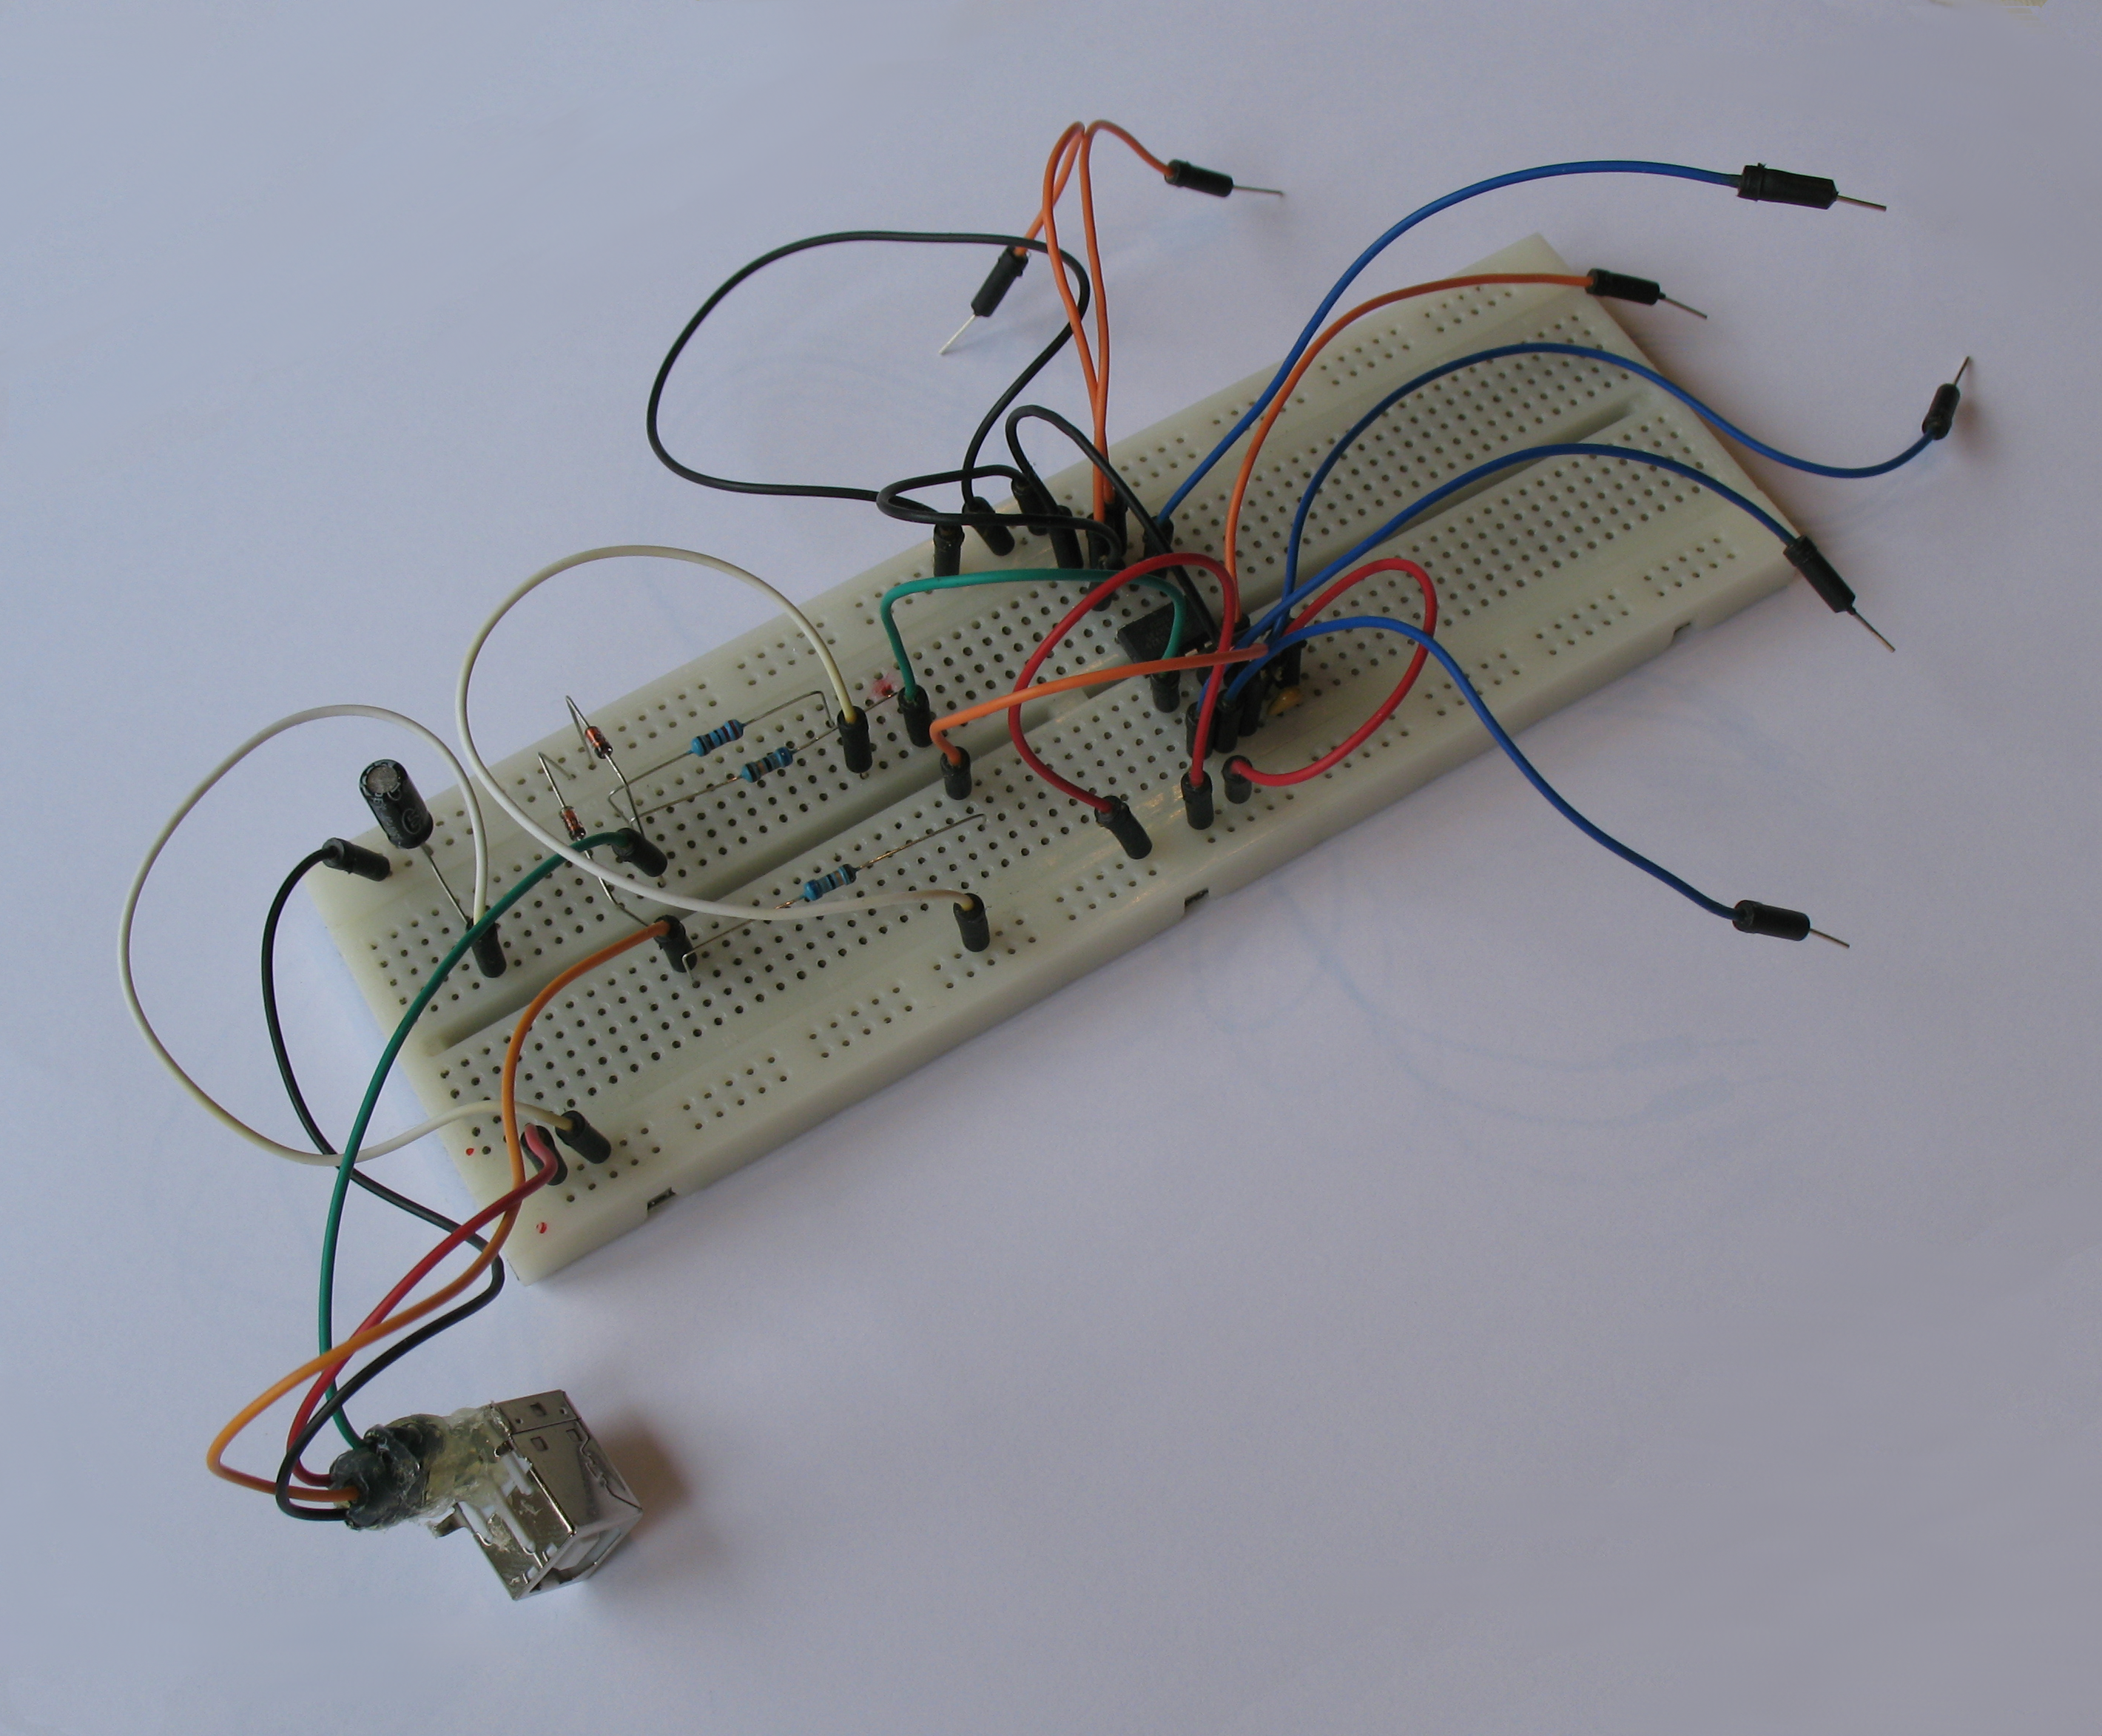
\includegraphics[width=\textwidth]{afbeeldingen/inputmodule_breadboard}
	\caption{Breadboard prototype.}
	\label{fig:breadboard}
\end{figure}

\section{Productie}

De finale stap bestaat eruit om het ontworpen schema te realiseren en een fysieke printplaat te laten maken, ofte een \ac{pcb}. Hierbij moeten we manueel een fysieke layout aanmaken en baantjes trekken waar er stroom moet kunnen vloeien. De plaatsing van die componenten is echter niet louter willekeurig. Zo is het bijvoorbeeld interessant om de componenten efficiënt te plaatsen zodat de uiteindelijke printplaat zo klein mogelijk is. Maar er zijn ook andere zaken waarmee we moeten rekening houden. Zo is er bijvoorbeeld de kwestie van plaatsing van de ontkoppelingscondesatoren: die worden best zo dicht mogelijk bij de bron van de spanningsoscillaties geplaatst.

Vooraleerst zijn we op zoek gegaan naar een fabrikant die voor een aanvaardbaar tarief een voldoende gesofisticeerde printplaat kan produceren. De mogelijkheden zijn eens te meer zeer uitgebreid, maar na een uitgebreide vergelijking zijn we terechtgekomen bij \makeurl{http://www.eurocircuits.com/}{Eurocircuits}, een Europees bedrijf met verschillende vestigingen, waaronder België. Hoewel de verschillen tussen andere fabrikanten niet al te groot zijn, heeft de combinatie van een competitieve prijs, beperkte verzendkosten, en verschillende positieve kritieken ons ertoe overtuigd om voor de diensten van Eurocircuits te kiezen.

Vervolgens hebben we een gekeken naar de eisen en mogelijkheden die het goedkoopste van de productietypes te vinden bij Eurocircuits - de standard pool - biedt. De \makeurl{http://www.eurocircuits.com/images/stories/ec09/ec-standard-pool-overview-english-1-2010-v3.pdf}{volledige lijst} is te uitgebreid om hier te vermelden, daarom halen we enkel de belangrijkste elementen aan:
\begin{itemize}
\item Maximaal 8 layers;
\item Top- en bottom solder mask;
\item Top- en bottom silkscreen.
\end{itemize}
Om de overige eisen, denk maar aan de minimale afstand tussen boorgaten of de minimale breedte van elektrische baantjes, te controleren zullen we gebruik maken van een \ac{dru} bestand. Dergelijke bestanden worden vaak aangeboden door te fabrikant, en laten toe om geautomatiseerd alle eisen te controleren die aan een printplaat gesteld worden.

Om een printplaat of printplaat te ontwerpen hebben we natuurlijk gepaste software nodig. De meest populaire keuze hierbij is de EAGLE PCB software, ontwikkeld door \makeurl{http://www.cadsoftusa.com/}{CadSoft}, waarschijnlijk omdat er een beperkte variant van de software gratis beschikbaar is. Wegens de populariteit van de tool bestaat er een heel actieve community, waardoor een zeer uitgebreide selectie aan componenten beschikbaar zijn voor gebruik binnen EAGLE. Ook biedt Eurocircuits enkel \ac{dru} bestanden aan voor de EAGLE software. Het lijkt daarom een verstandige keuze om onze printplaat ook te ontwerpen met EAGLE.

Nu we alle nodige specificaties vergaard hebben en een softwarepakket geselecteerd hebben, kunnen we beginnen aan het produceren van de fysieke layout. Hierbij hebben we ervoor gekozen om een printplaat te maken die bestaat uit twee lagen, namelijk de boven en onderkant. Deze optie is niet veel duurder dan een 1-laags printplaat, en het geeft ons de nodige flexibiliteit om de componenten goed te kunnen plaatsen. Moesten we gekozen hebben voor een 1-laags printplaat dan zou de kost misschien zelfs hoger kunnen liggen door soms onnatuurlijke plaatsing om toch de nodige verbindingen te kunnen realiseren. 

De finale versie van de 2-laags printplaat is te vinden in figuur \ref{fig:printplaat}. Hierbij zijn een aantal zaken waard om te vermelden. Zo is er de plaatsing van de 100 nanofarad condensator die instaat voor het ontkoppelen van de hoogfrequente ruis: aangezien dergelijke ruis veroorzaakt wordt door het schakelen van de transistoren binnen de microcontroller, hebben we de condensator zo dicht mogelijk geplaatst bij de bron van die ruis. Ook hebben we zoals de gewoonte is bij het ontwerpen van een schema, de vrije ruimte van elke laag gebruikt om een volledig geleidend vlak te maken. Daarbij zal de fill op de bovenste layer gebruikt worden om de positieve voedingsspanning $Vcc$ te geleiden, en de fill op de onderste layer om de elektronische grond te verdelen. Hoewel dit bij een hoogfrequent-circuit niet zou aan te raden zijn wegens de parasitaire capaciteiten die gepaard gaan met dergelijke \emph{plane fills}, is dit bij ons relatief laagfrequent schema niet van toepassing.

\begin{figure}
	\includegraphics[width=\textwidth]{afbeeldingen/inputmodule_pcb}
	\caption{Finale versie van de printplaat.}
	\label{fig:printplaat}
\end{figure}

De laatste stap voor de effectieve productie is de conversie van ons schema naar het bestandsformaat dat vereist is door Eurocircuits. Hoewel dit verschilt van producent tot producent, moeten we meestal voorzien in de volgende bestanden (met het formaat steeds tussen haakjes):
\begin{itemize}
  \item Top copper (Extended Gerber): koper op bovenste laag;
  \item Bottom Copper (Extended Gerber): koper op onderste laag;
  \item Top Silkscreen (Extended Gerber): tekst op bovenste laag;
  \item Top Soldermask (Extended Gerber): plaatsen op bovenste laag die moeten bedekt worden met beschermende laag;
  \item Bottom Soldermask (Extended Gerber): plaatsen op bovenste laag die moeten bedekt worden met beschermende laag;
  \item Drill File (Excellon): waar en hoe er geboord moet worden op de printplaat.
\end{itemize}

Het genereren van deze bestanden kunnen we uitvoeren met Eagle's CAM Processor. Hiertoe hebben we ons gebaseerd op een voorbeeld CAM job van Sparkfun, aangepast aan de specifieke eisen die Eurocircuit stelt. Na het insturen van deze bestanden, selectie van de benodigde materialen en processen, kregen we na enkele weken een afgewerkte printplaat in de bus. Vervolgens zijn we overgegaan tot aankoop van de benodigde componenten, waarna we die er op gesoldeerd hebben om dan eindelijk een afgewerkte print te bekomen zoals te zien in figuur \ref{fig:inputmodule}.

\begin{figure}
	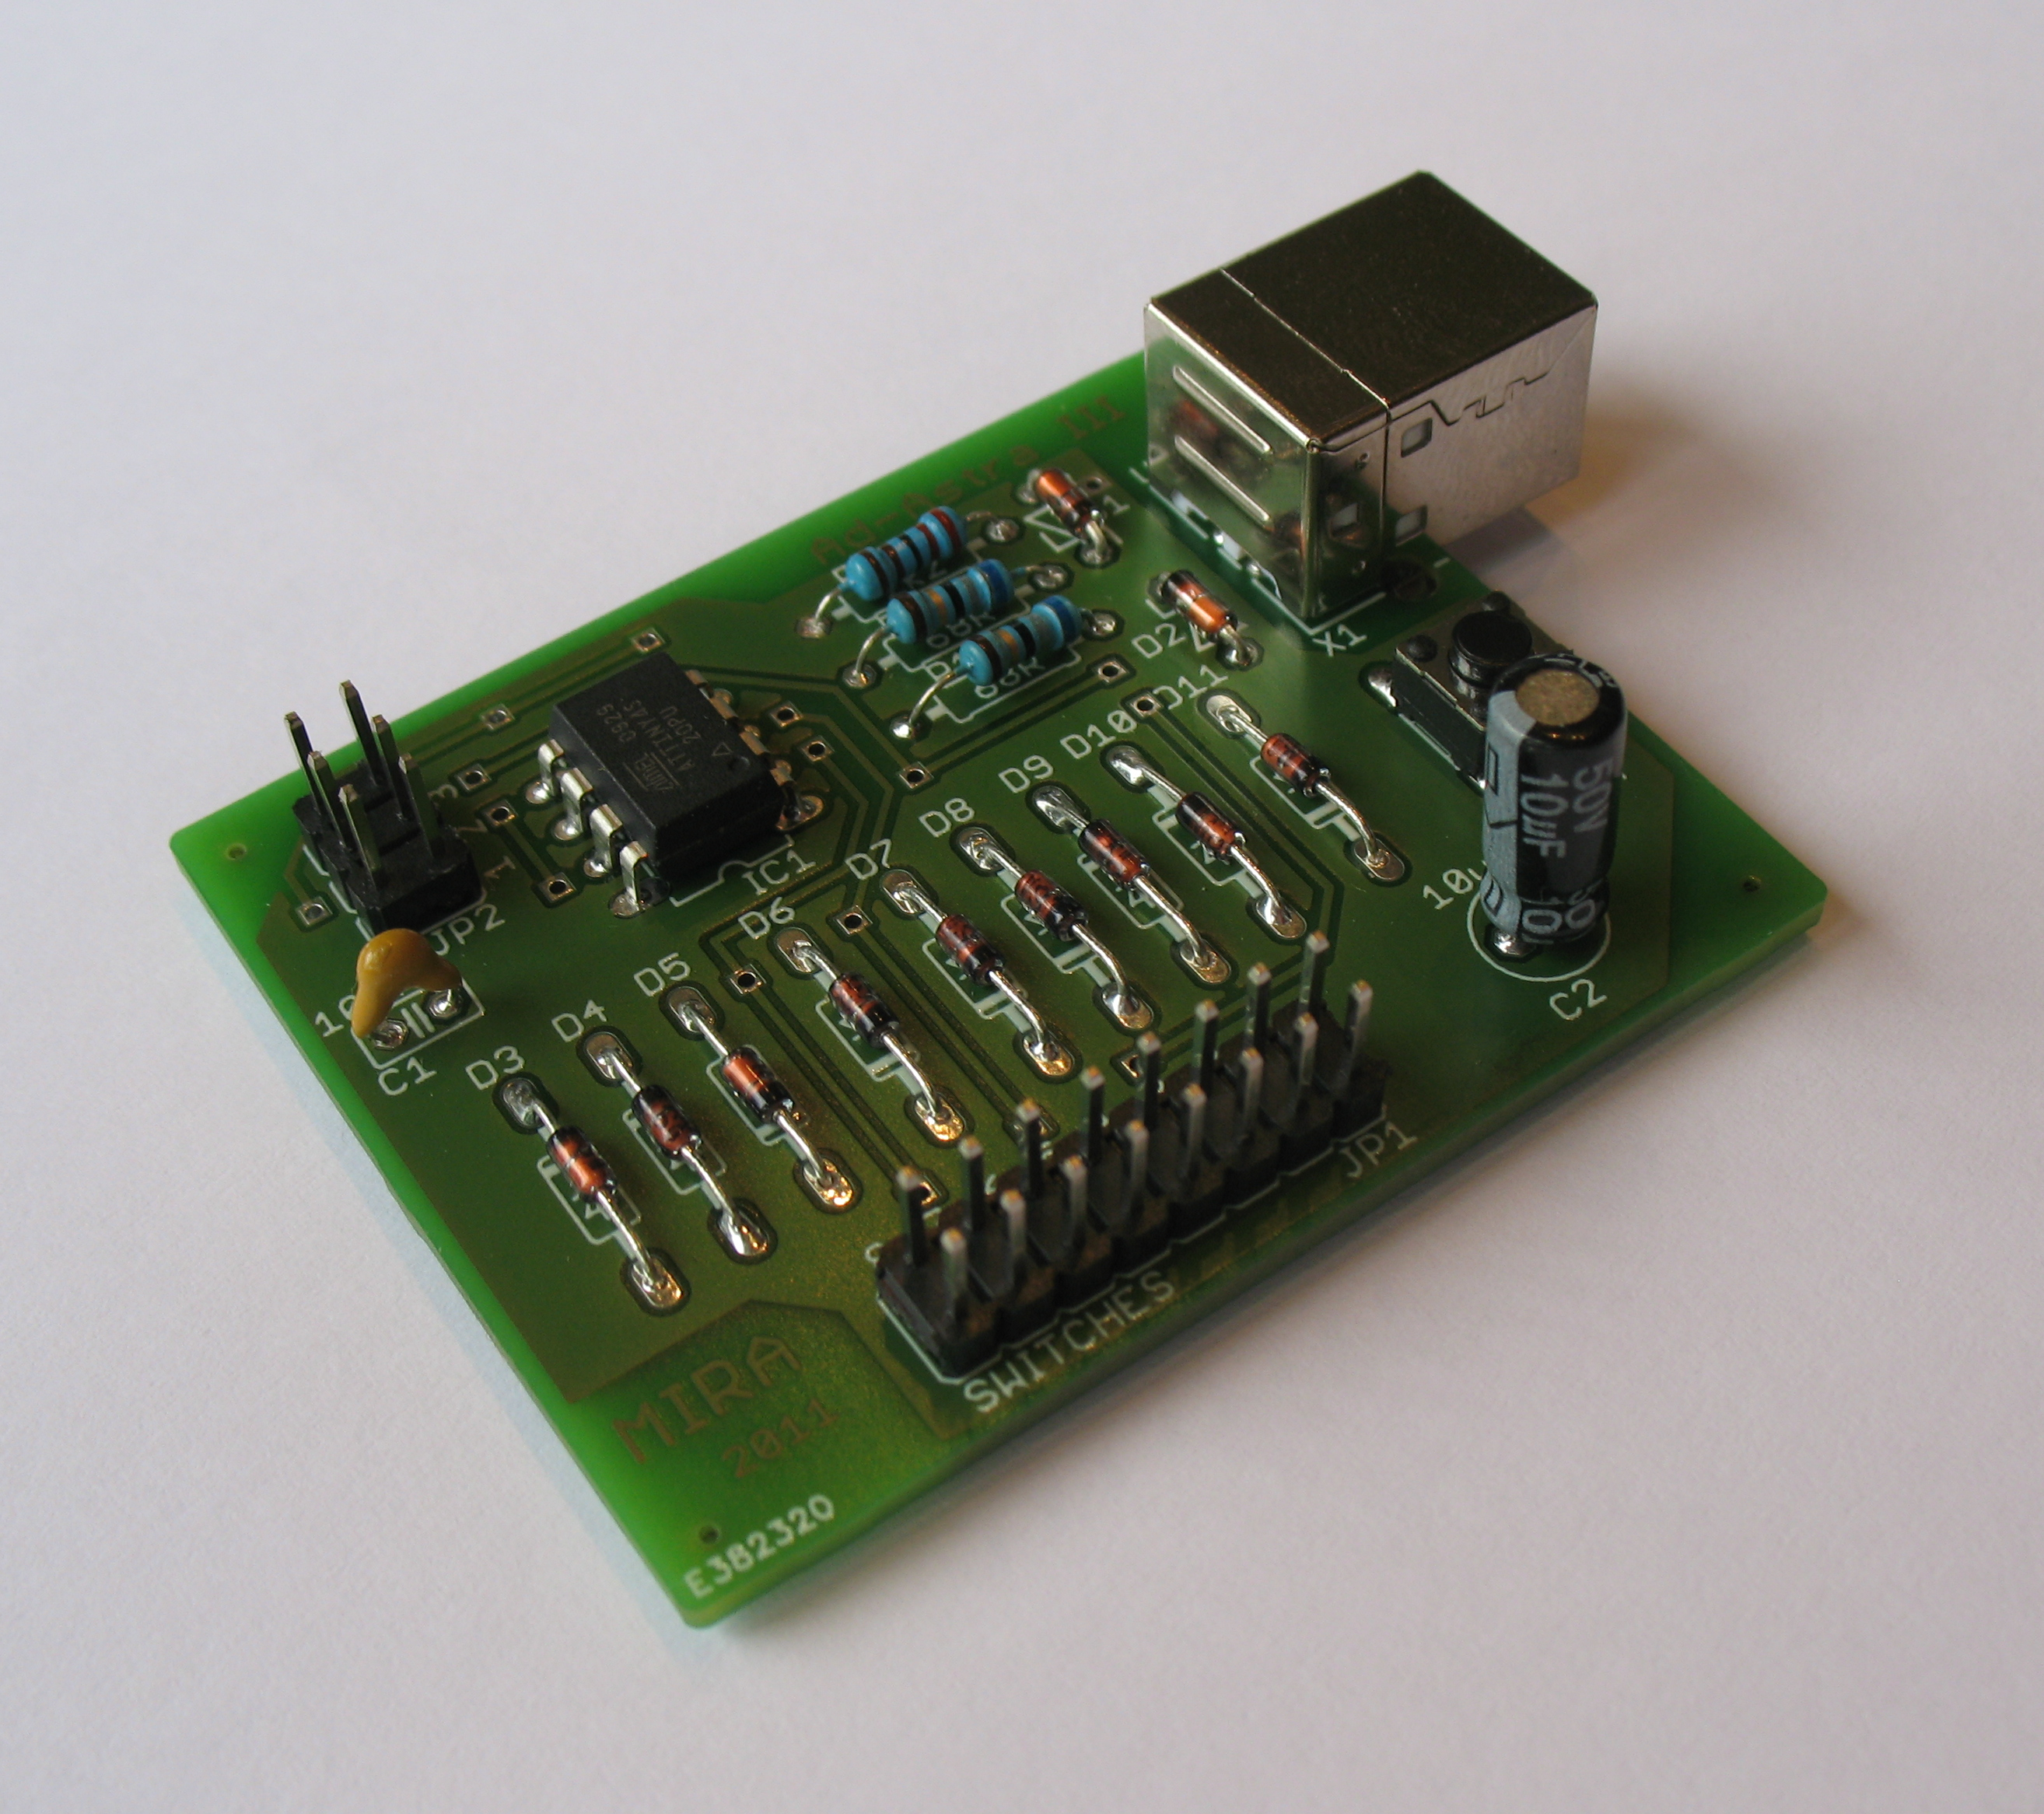
\includegraphics[width=\textwidth]{afbeeldingen/inputmodule_afgewerkt}
	\caption{Finale versie van de inputmodule.}
	\label{fig:inputmodule}
\end{figure}


\chapter{Firmware}

\section{Geheugengebruik}

Bij het schrijven van de firmware moesten we rekening houden met de mogelijkheden van de chip. Deze eigenschappen, vermeld in sectie \ref{inputmodule:hardware:microcontroller}, waren vaak sterk beperkend. Zo hadden we maar 4 kilobytes tot onze beschikking, waardoor het moeilijk zou worden om (een subset van) C++ te gebruiken: de overhead teweeggebracht door het gebruik van klassen is immers te groot. Ook moesten we erop letten om geen \emph{floating-point} berekeningen uit te voeren: aangezien de AtTiny45 geen \ac{fpu} bevat, zou het gebruik ervan resulteren in het meelinken van een \ac{fpu}-emulator (die ruim 2 kilobytes groot is).

Ook moeten we rekening houden met de beperkte hoeveelheid \ac{ram} geheugen. Een voorbeeld van een dergelijke optimalisatie is hoe we 14 bytes \ac{ram} geheugen uitgespaard hebben bij de lookup-table waarmee een bitmap van geactiveerde schakelaars geconverteerd wordt naar de geschikte toetsaandruk. Aangezien we over 7 schakelaars bevatten, en er 1 extra entry in de lookup tabel aanwezig is voor wanneer er geen toets ingedrukt is, hebben we 8 ingangen nodig binnen de lookup-table. Voor elke ingang in die tabel, die we indexeren met de bitmap om zo geen extra ruimte te vereisen, hebben we twee waarden nodig: de toets, en een modifier (zoals \code{shift} of \code{alt}). Beide waarden worden geëncodeerd als een \code{uchar}, en nemen dus elk 1 byte in beslag. Hierdoor is de hele lookup-table exact 16 bytes groot. Omdat we deze tabel rechtstreeks indexeren moet ze volledig in het \ac{ram} geheugen staan, zélfs als we ze nooit zullen wijzigen. Om deze verkwisting te vermijden zullen we gebruik maken van de \code{PROGMEM} macro die ons toelaat om bepaalde datastructuren onder dwang in het programmageheugen op te slaan. Hoewel we daardoor 16 bytes uitsparen, moeten we nu meer opletten bij het gebruik van de lookup-tabel: de tabel is niet langer rechtstreeks te indexeren. Meer concreet: pointers die we berekenen door het optellen van een offset (de bitmap waarmee we normaal de tabel indexeerden) met het basisadres van de tabel mogen we nu niet langer rechtstreeks dereferentieren, maar enkel na aanroepen van de \code{pgm\_read\_word} functie. Het resultaat, nu slechts 2 bytes groot, dienen we natuurlijk op te slaan in \ac{ram} geheugen.

\begin{lstlisting}[language=C, float, caption=Optimalisatie van de lookup-table.]
static const uchar keyReport[NUM_KEYS+1][2] PROGMEM = {
/* none */  {0, 0},
/*  1 */    {MOD_SHIFT_RIGHT, KEY_1},
/*  2 */    {MOD_SHIFT_RIGHT, KEY_2},
/*  3 */    {MOD_SHIFT_RIGHT, KEY_3},
/*  4 */    {MOD_SHIFT_RIGHT, KEY_4},
/*  5 */    {MOD_SHIFT_RIGHT, KEY_5},
/*  6 */    {MOD_SHIFT_RIGHT, KEY_6},
/*  7 */    {MOD_SHIFT_RIGHT, KEY_7},
};

static void handleKeyPress(uchar key)
{
    *(int *)data = pgm_read_word(keyReport[key]);
}
\end{lstlisting}

Tenslotte gebruiken we ook nog 1 byte uit het \ac{eeprom} geheugen om het resultaat van een succesvolle calibratie in op te slaan. Die calibrarie is, zoals beschreven in sectie \ref{inputmodule:hardware:microcontroller}, nodig omdat we geen oscillator gebruikt hebben op de printplaat. Omdat die calibratie echter enige tijd in beslag neemt, slaan we het resultaat ervan op zodat na een heropstart de calibratie niet opnieuw moet uitgevoerd worden.

Na verschillende optimalisaties ziet het geheugengebruik er als volgt uit:
\begin{table}[h!]
  \begin{center}
    \begin{tabular}{c c c}
    Geheugen & Gebruik & Limiet \\
    \hline
    Flash & 2172 bytes & 4 kilobytes \\
    \ac{ram} & 61 bytes & 256 bytes \\
    \ac{eeprom} & 1 byte & 256 bytes \\
    \end{tabular}
  \end{center}
  \caption{Geheugengebruik van de firmware voor de inputmodule.}
\end{table}

\section{Codeanalyse}
\label{inputmodule:firmware:codenalyse}

Net zoals we bij de kioskapplicatie een probleem hadden om de constructies specifiek aan Qt te analyseren, was het ook niet eenvoudig de code van de firmware te controleren. Het probleem hierbij is dat de code opnieuw gebruik maakt van een groot aantal macro's en symbolen gedefiniëerd door een complexe combinatie van AVR-specifieke headers en symbolen die via de command-line aan de preprocessor doorgegeven worden. Om dit te illustreren leggen we uit hoe je een bit uitschrijft naar de eerste pin van de eerste uitwendige poort. De code daarvoor is eenvoudig, en werkt op alle AVR microcontrollers: \code{PORTA = (1<<PA1);}. Hierbij zijn er twee speciale symbolen in het spel: \code{PORTA} die naar de juiste I/O-registers van de poort wijst, en \code{PA1} die indiceert hoeveel plaatsen de bit moet opgeschoven worden om terecht te komen op het gedeelte van het I/O-register dat wijst naar de eerste pin van de poort.

Het is duidelijk dat exacte inhoudt van deze registers verschilt van model tot model, en die symbolen gebruikt worden om de code enigszinds overdraagbaar te houden. Wanneer de code echter gecompileerd wordt, moeten deze symbolen vervangen worden door de juiste geheugenadressen en waarden. Daarvoor zorgen de headers uit de AVR C-library, tegelijk een mooie illustratie van de mogelijkheden die de C preprocessor biedt. Een illustratief voorbeeld van hoe de het \code{PA1} symbool door de preprocessor zal omgezet worden, is zien in fragment \ref{lst:avr:preprocessor}.

\begin{lstlisting}[language=C, float, caption=Omzetten van AVR symbolen via preprocessor-logica., label=lst:avr:preprocessor]
#ifndef _AVR_ATTINY13A_
  #define PA1 2
  #define PA2 1
  #define PA3 0
#elif _AVR_ATTINY45PU_
  #define PA1 0
  #define PA2 1
  #define PA3 2
  #define PA4 4
#else
  #error Unknown microprocessor model.
#endif
\end{lstlisting}

Zoals te zien is in fragment \ref{lst:avr:preprocessor} berust de preprocessor op enkele symbolen die door de programmeur moeten gespecificeerd worden. Die symbolen moeten gedefiniëerd zijn wanneer de preprocessor de code verwerkt, wat in de praktijk vaak gedaan wordt door een header te includen (bijvoorbeeld \code{settings.h}) die als enige taak heeft die kritieke symbolen te definiëren. Wij hebben er echter voor gekozen om de symbolen door te geven aan de compiler en preprocessor via de command-line, waardoor we alle configuratie kunnen isoleren binnen de \code{Makefile}.

Het grote probleem met al deze preprocessor-logica is dat statische analyse-tools er vaak niet goed mee overweg kunnen. Het is ook geen oplossing om eerst de preprocessor zijn werk te laten doen omdat de code dan vaak niet meer herkenbaar is en het voor de programmeur dan niet te doen is om de output van de analysetools correct te interpreteren. Daarom hebben we, zeker gezien de beperkte grootte van de firmware (nog geen 250 regels code) besloten om niet verder te zoeken naar analysetools en gewoon zelf de code eens extra grondig te controleren.

\section{Compilatie}

Het grote probleem bij het compileren van de firmware is dat de machinecode die de AVR microcontroller vereist niet compatibel is met de x86-machinecode die een compiler op onze computers genereerd. We zullen dus een compiler moeten gebruiken die specifiek geconfigureerd is om machinecode te genereren die kan draaien op een ander systeem dan hetgene waar de compiler op uitgevoerd wordt. Dit proces heet \emph{cross compiling}.

Als we kijken naar de bekendere open-source compilers is de AVR port van \ac{gcc} de de-facto standaard voor het compileren van code voor AVR microprocessoren. Ook zou het gebruiken van een andere compiler ervoor zorgen dat we flink wat code zouden moeten converteren om uberhaupt nog te compileren. Veel van de preprocessor-logica beschreven in sectie \ref{inputmodule:firmware:codenalyse} is immers geïmplementeerd met \ac{gcc}-specifieke instructies (ook wel \emph{compiler intrinsics} genoemd). Als we bijvoorbeeld naar een andere kwalitatieve compiler kijken, IAR's Embedded Workbench, moeten we zelf afhankelijk van het model microprocessor bepalen welke header we gebruiken, en is het natuurlijk niet mogelijk om daarvoor de \ac{gcc} headers te gebruiken die wel voorzien in een handige abstractielaag.

Om tenslotte toch nog enigszinds aan codeanalyse te doen hebben we vervolgens \ac{gcc} dusdanig geconfigureerd dat het zoveel mogelijk potentiële fouten detecteerd en uitschrijft. Dit hebben we gedaan met de \code{-Wall} en \code{-Wextra} parameters, waarmee we een probleem hebben ondekt betreffende \emph{pointer aliasing}.

\part{Voorstellingen}
\label{voorstellingen}

\textit{Dummy tekst omdat \LaTeX anders zot komt.}


\appendix

\backmatter
% Bibliografie
\bibliographystyle{plainnat}
\bibliography{verslag}


\end{document}
